\documentclass[12pt, titlepage]{article}

\usepackage{amsmath, mathtools}
\usepackage{amsfonts}
\usepackage{amssymb}
\usepackage{colortbl}
\usepackage{xr}
\usepackage{hyperref}
\usepackage{longtable}
\usepackage{xfrac}
\usepackage{tabularx}
\usepackage{siunitx}
\usepackage{caption}
\usepackage{pdflscape}
\usepackage{afterpage}
\usepackage{verbatim}
\usepackage[round]{natbib}
\usepackage{colortbl}
\usepackage{hyperref}
\usepackage{lingmacros}
\usepackage{tree-dvips}
\usepackage{blindtext}
\usepackage{colortbl}%For FR tables
\usepackage{hyperref}%For advanced hyperlinks
\usepackage{enumitem}%For advanced lists
\usepackage{pdfpages}
\usepackage{array}
\usepackage{tikz}
\usepackage{pdflscape}

\usepackage{fullpage}
\usepackage{multirow}
\usepackage{booktabs}
\usepackage{graphicx}
\usepackage{float}
\usepackage{ulem}
\usepackage[many]{tcolorbox}
\newtcolorbox{cross}{blank,breakable,parbox=false,
  overlay={\draw[red,line width=5pt] (interior.south west)--(interior.north east);
    \draw[red,line width=5pt] (interior.north west)--(interior.south east);}}

\usepackage[toc,page]{appendix}
\hypersetup{
    colorlinks,
    citecolor=blue,
    filecolor=black,
    linkcolor=red,
    urlcolor=blue
}

%% Comments

\usepackage{color}

\newif\ifcomments\commentstrue %displays comments
%\newif\ifcomments\commentsfalse %so that comments do not display

\ifcomments
\newcommand{\authornote}[3]{\textcolor{#1}{[#3 ---#2]}}
\newcommand{\todo}[1]{\textcolor{red}{[TODO: #1]}}
\else
\newcommand{\authornote}[3]{}
\newcommand{\todo}[1]{}
\fi

\newcommand{\wss}[1]{\authornote{blue}{SS}{#1}} 
\newcommand{\plt}[1]{\authornote{magenta}{TPLT}{#1}} %For explanation of the template
\newcommand{\an}[1]{\authornote{cyan}{Author}{#1}}

%% Common Parts

\newcommand{\progname}{ProgName} % PUT YOUR PROGRAM NAME HERE
\newcommand{\authname}{Team \#, Team Name
\\ Student 1 name
\\ Student 2 name
\\ Student 3 name
\\ Student 4 name} % AUTHOR NAMES                  

\usepackage{hyperref}
    \hypersetup{colorlinks=true, linkcolor=blue, citecolor=blue, filecolor=blue,
                urlcolor=blue, unicode=false}
    \urlstyle{same}
                                


\newcounter{acnum}
\newcommand{\actheacnum}{AC\theacnum}
\newcommand{\acref}[1]{AC\ref{#1}}

\newcounter{ucnum}
\newcommand{\uctheucnum}{UC\theucnum}
\newcommand{\uref}[1]{UC\ref{#1}}

\newcounter{mnum}
\newcommand{\mthemnum}{M\themnum}
\newcommand{\mref}[1]{M\ref{#1}}

\begin{document}

\title{System Design: \progname{}} 
\author{\authname}
\date{\today}

\maketitle

\pagenumbering{roman}

\section*{Revision History}

\begin{tabularx}{\textwidth}{p{3cm}p{2cm}X}
\toprule {\bf Date} & {\bf Version} & {\bf Notes}\\
\midrule
January 15 & 1.0 & Added Template \\
January 16 & 1.1 & Added sections 1, 2, 3\\
January 17 & 1.2 & Added sections 4, 5, 6\\
January 18 & 1.3 & Added sections 7, 8, 9, 10, Appendices\\
April 5 & 1.4 & Updated for feedback and consistency\\
\bottomrule
\end{tabularx}

\newpage

\section*{Reference Material}

This section records information for easy reference.

\subsection*{Abbreviations and Acronyms}

\renewcommand{\arraystretch}{1.2}
\begin{tabular}{l l} 
  \toprule		
  \textbf{symbol} & \textbf{description}\\
  \midrule 
  \progname & Explanation of program name\\
  \bottomrule
\end{tabular}\\

\newpage

\tableofcontents

\newpage

\listoftables

\listoffigures

\newpage

\pagenumbering{arabic}

\section{Introduction}
Synesthesia Wear is a wearable \sout{product} \textcolor{red}{device} that \sout{assists users with certain vocal tasks 
that need attention. These tasks can be generic or custom to the user as needed.} \textcolor{red}{improves users' auditory awareness of their surroundings.}
Furthermore, the product will use signal processing to gather and analyze information 
to determine the best and most appropriate feedback (via vibrations) to send to the 
user. As a result, this gives the users peace of mind knowing that if their attention 
is needed (doorbell, ring, name call, etc.), Synesthesia Wear will be able to alert them.

\section{Purpose}
The purpose of this document is to be able to identify and elaborate on all aspects of design involved
in the creation of the Synesthesia Wear system. This involves decomposing the system into different categories and components 
that all have an impact on the system's overall design and functionality.

To add on, this document is intended to be viewed in conjunction with the \href{https://github.com/jordanbierbrier/capstone/blob/main/docs/Design/SoftArchitecture/MG.pdf}{\textit{MG.pdf}} (Software Architecture Design) 
and the \href{https://github.com/jordanbierbrier/capstone/blob/main/docs/Design/SoftDetailedDes/MIS.pdf}{\textit{MIS.pdf}} (Detailed Design) documents so that readers may have a full comprehension on the many aspects of Synesthesia 
Wear's design in its entirety. 

\section{Scope}
\subsection {Document Scope}
As stated before, this document will split up the system design into different categories and components 
such that the readers may be able to better understand each components impact on the system's functionality/completeness.\\\\
\noindent With the above in mind, the scope of this document will involve:
\begin{itemize}
  \item \textbf{Project Overview:} This section goes over the system's behaviour, undesired event handling, system components, and requirement-design connections.  
  \item \textbf{System Variables:} As its name suggests, this section goes over variables/aspects to the system that has the potential to change.
  \item \textbf{User Interfaces:} This section involves elaborating on the interfaces that users interact with when using the Synesthesia Wear system.
  \item \textbf{Design of Mechanical Hardware:} In this section, details on what will be built, fabrication, materials, and drawings/sketches for mechanical components will be discussed in further detail. 
  \item \textbf{Design of Electrical Components:} Similar to design of hardware, this section will instead involve details regarding electrical components.
  \item \textbf{Design of Communication Protocols:} For this section, details on the communication protocols used in the Synesthesia Wear system will be discussed.
  \item \textbf{Timeline:} This section will go over the schedules of all remaining tasks for Rev 0 and which team member will be responsible for each task's completion.
\end{itemize}

\subsection {Assumptions}
The system is designed with the following assumptions:
\begin{table}[H]
  \centering
  \arrayrulecolor{white}
  \begin{tabular}{|p{3cm}|p{11cm}|} 
  \hline
  \rowcolor[rgb]{0.071,0.49,0.698} \textcolor{white}{A1} & \textcolor{white}{Each user has a device and WIFI capable of installing the Synesthesia Wear application.}                                          \\ 
  \hline
  \rowcolor[rgb]{0.675,0.827,0.902} Rationale               & Without a device and/or internet connection, the user will be unable to benefit from using Synesthesia Wear.\\
  \hline
  \end{tabular}
  \arrayrulecolor{black}
\end{table}

\begin{table}[H]
  \centering
  \arrayrulecolor{white}
  \begin{tabular}{|p{3cm}|p{11cm}|} 
  \hline
  \rowcolor[rgb]{0.071,0.49,0.698} \textcolor{white}{A2} & \textcolor{white}{The users set their sound configurations to realistic daily-life sounds.}                                    \\ 
  \hline
  \rowcolor[rgb]{0.675,0.827,0.902} Rationale               & The system would be inaccurate when trying to process \quad imaginary or rare sounds with a lack of audio samples (like a meteor crash).\\
  \hline
  \end{tabular}
  \arrayrulecolor{black}
\end{table}

The following are in reference to the critical assumptions in Synesthesia Wear's

\href{https://github.com/jordanbierbrier/capstone/blob/main/docs/HazardAnalysis/HazardAnalysis.pdf}{\textit{HazardAnalysis.pdf}} document:

\begin{table}[H]
  \centering
  \arrayrulecolor{white}
  \begin{tabular}{|p{3cm}|p{11cm}|} 
  \hline
  \rowcolor[rgb]{0.071,0.49,0.698} \textcolor{white}{A3} & \textcolor{white}{The battery will not need to be replaced during product \quad lifespan.}                                          \\ 
  \hline
  \rowcolor[rgb]{0.675,0.827,0.902} Rationale               & It is undesirable and annoying for users if they had to replace the battery frequently during use.\\
  \hline
  \end{tabular}
  \arrayrulecolor{black}
\end{table}

\begin{table}[H]
  \centering
  \arrayrulecolor{white}
  \begin{tabular}{|p{3cm}|p{11cm}|} 
  \hline
  \rowcolor[rgb]{0.071,0.49,0.698} \textcolor{white}{A4} & \textcolor{white}{The microphone is not blocked and has realistic access to the environment.}                                          \\ 
  \hline
  \rowcolor[rgb]{0.675,0.827,0.902} Rationale               & If the microphone is intentionally blocked or put into an environment that hinders its detection (anechoic chamber), it is unreasonable to expect accurate results.\\
  \hline
  \end{tabular}
  \arrayrulecolor{black}
\end{table}




\subsection {System Context}
\begin{figure}[H]
  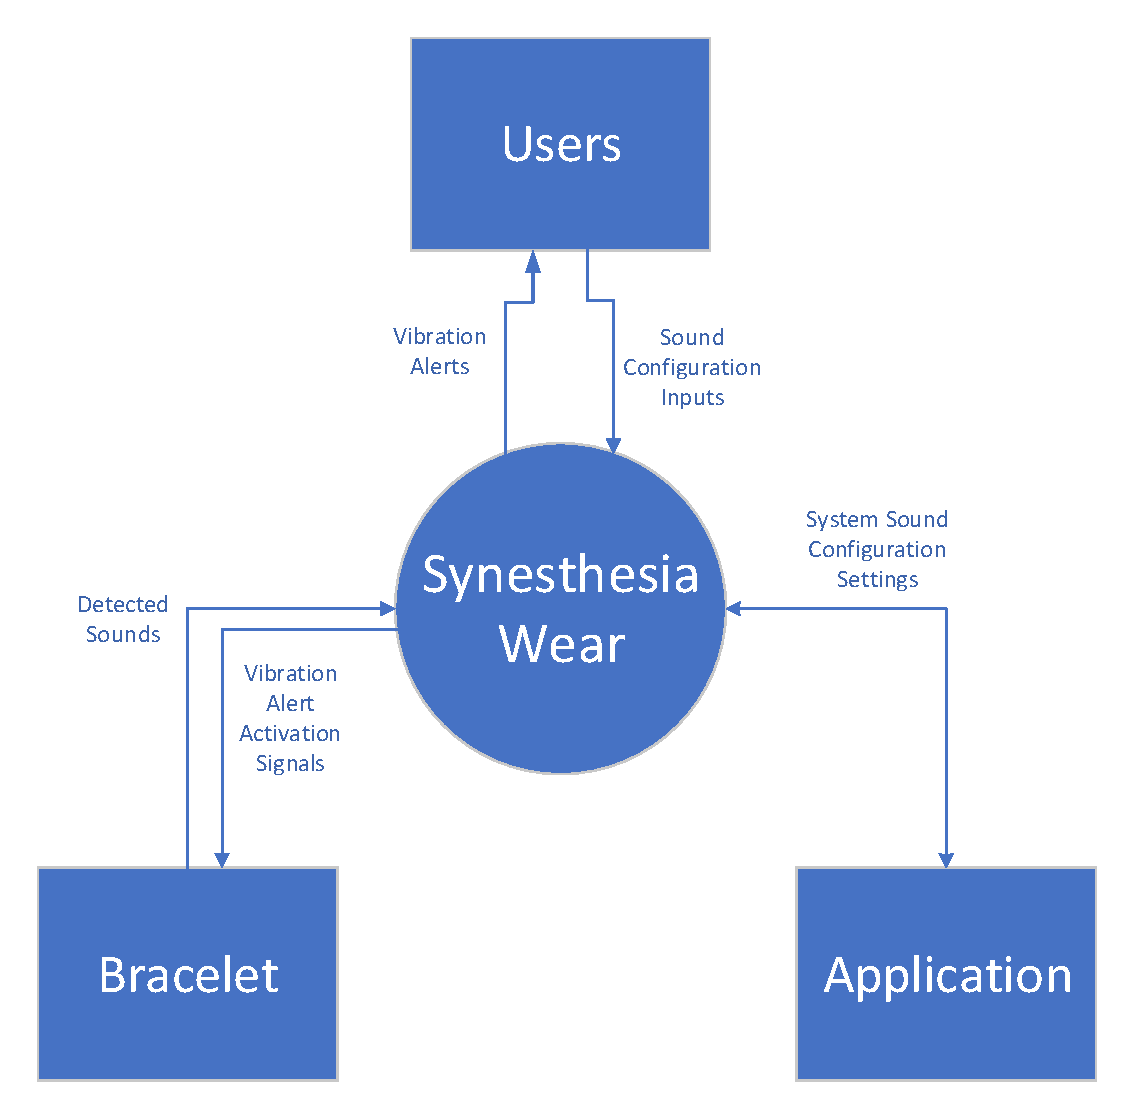
\includegraphics[width=\textwidth,height=\textheight,keepaspectratio]{ContextDiagram.pdf}
  \caption{System Context Diagram}
  \label{ContextDiagram} 
\end{figure}

\section{Project Overview}

\subsection{Normal Behaviour}
When starting off, the users should strap the Synesthesia Wear bracelet onto either of their wrists as it was intended.
Afterwards, users would have to install the Synesthesia Wear app onto a device of their choice and possibly look through the app 
to get more familiar with its features and user interface. When ready, the user would then input their desired sound configuration 
settings into the app and then save them so that the app can send these settings over to the bracelet for configurations.
Once recieved, the bracelet can then start to detect for sounds where its built-in microcontroller will process these sounds and try to 
match it with the sounds configured in the settings. Lastly, once a detected sound has ``accurately'' (according to Machine Learning Algorithm) matched a configured sound, a vibration 
alert signal will be sent to the built-in vibration motor which will notify the user that their attention is needed.

\subsection{Undesired Event Handling}
Currently, there are only a few undesired events that can be indentified. However, as time progresses, more undesired events will be recognized and dealt with appropriately. 
So for now, any undesired events not yet discovered will be resolved by setting the Synesthesia Wear system into a dormant state and alerting the user. This makes it so that potential system issues are prevented while also keeping the user informed that the system is in a dormant state and needs a reset for continued use. \\ \\ 
With the above in mind, an undesired event that has been identified is in regards to the bracelet trying to detect/process sounds before sound configuration settings have been set.
To deal with this, similar to unidentified events, the Synesthesia Wear system will be created such that it is in a dormant/inactive state until sound configuration settings have been inputted.
However, one exception would be that there is no need to alert the user for a reset since they have just started using Synesthesia Wear in its refreshed/new state. \\\\
Another undesired event would be in regards to the components breaking or malfunctioning. In these cases, the system will be made such that it tests connections/signals between components (like microncontroller, application, etc.) and alerts the user when a connection test has consistently failed.
Afterwards, the user would need to contact the Synesthesia Wear team and they would then try to fix the components or order new parts to replace the broken ones. \\\\
A third undesired event would be in regards to intentionally covering/hindering the bracelet to detect sounds via holding the bracelet or going into a anechoic (soundless) chamber.
In this situation, the microphone in the bracelet will be unable to accurately detect sounds in the environment while its functionality is obstructed. With this in mind, it is believed that there is not really any resolution needed for this situation considering once the user reenters a ``normal'' or unhindered environment, so long as the components are undamaged, the system's functionality should still work as intended. 


\subsection{Component Diagram}
\begin{figure}[H]
  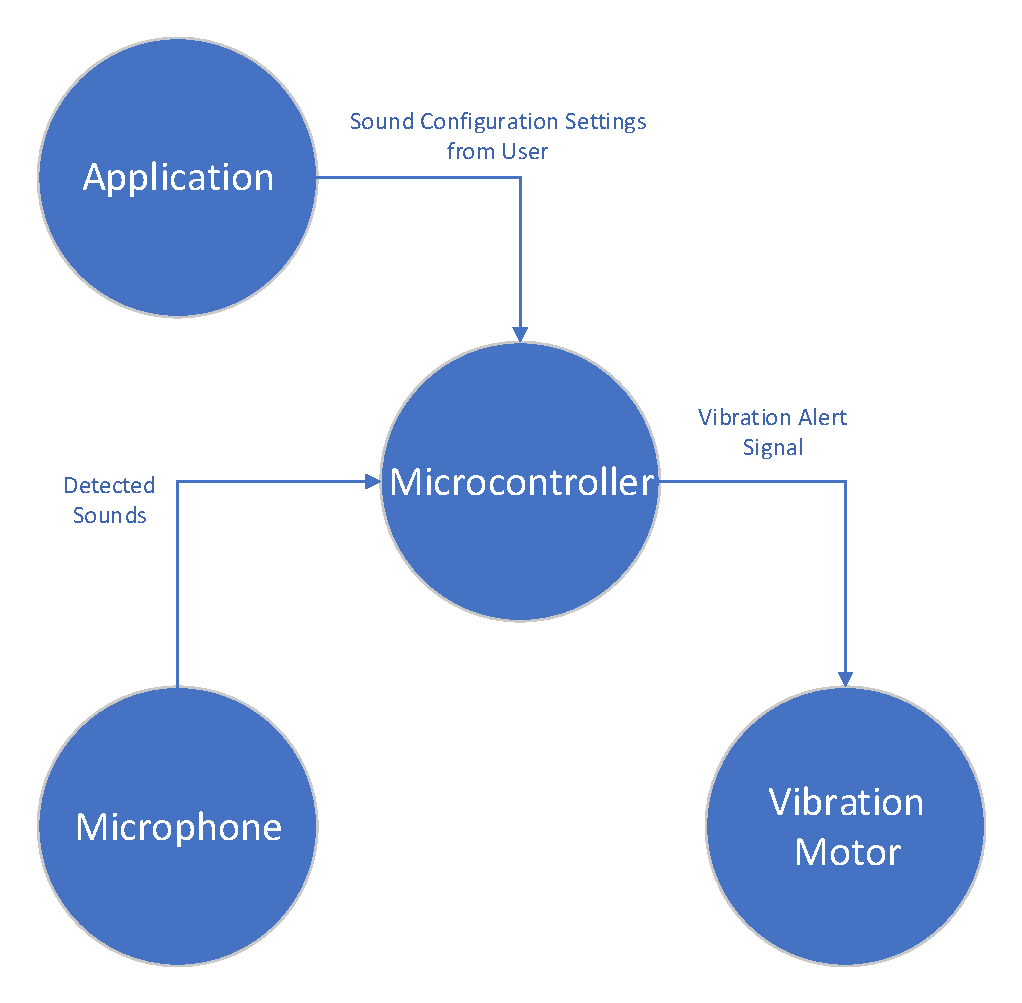
\includegraphics[width=\textwidth,height=\textheight,keepaspectratio]{ComponentDiagram.pdf}
  \caption{Component Diagram}
  \label{ComponentDiagram} 
\end{figure}

\subsection{Connection Between Requirements and Design} \label{SecConnection}

The following requirements were taken from Synesthesia Wear's
\href{https://github.com/jordanbierbrier/capstone/blob/main/docs/SRS/SRS.pdf}{\textit{SRS.pdf}} document:

\begin{table}[H]
  \centering
  \caption{Requirements and Design Connections Table}
  \label{table:Connections Table} 
  \arrayrulecolor{white}
  \begin{tabular}{|p{7cm}|p{7cm}|} 
  \hline
  \rowcolor[rgb]{0.071,0.49,0.698} \textcolor{white}{Requirements} & \textcolor{white}{Design Decision}                                          \\ 
  \hline
  \rowcolor[rgb]{0.675,0.827,0.902} Capability to pick up sounds.              & Need to purchase and integrate a microphone.\\
  \hline
  \rowcolor[rgb]{0.675,0.827,0.902} Capability to classify different sounds.              & Need to purchase and integrate a programmable microcontroller that can run machine learning classification algorithms.\\
  \hline
  \rowcolor[rgb]{0.675,0.827,0.902} Ability to set/change sound classifications.            & Need to create an application that allows users to change classification settings.\\    
  \hline
  \rowcolor[rgb]{0.675,0.827,0.902} Ability to effectively give the user feedback on a sound classification match.           & Need to purchase and integrate a vibration motor into the Synesthesia Wear bracelet.\\
  \hline
  \rowcolor[rgb]{0.675,0.827,0.902} Battery of the device should be shielded to prevent any direct contact with the user.           & Need to design/build/purchase a case around the bracelet where the battery will be stored to prevent damage and any contact between user and battery.\\
  \hline
  \rowcolor[rgb]{0.675,0.827,0.902} The product dimensions should allow fitment on wrist of the user.           & Need to purchase and integrate a \textcolor{red}{small} microcontroller with built-in modules (bluetooth, microphone, etc.) \sout{to reduce product dimensions} \textcolor{red}{such that the product dimensions are reduced} as much as possible.\\
  \hline
  \end{tabular}
  \arrayrulecolor{black}
\end{table}

\section{System Variables}
\subsection{Monitored Variables}
\begin{table}[H]
  \centering
  \caption{Monitored Variables Table}
  \label{table:MonitoredVar Table} 
  \arrayrulecolor{white}
  \begin{tabular}{|p{5cm}|p{5cm}|p{5cm}|} 
  \hline
  \rowcolor[rgb]{0.071,0.49,0.698} \textcolor{white}{Monitored Name} & \textcolor{white}{Monitored Type} & \textcolor{white}{Description}                                          \\ 
  \hline
  \rowcolor[rgb]{0.675,0.827,0.902}   detectedSounds      & Sound &  Sounds in the environment are being monitored and collected via a microphone in the Synesthesia Wear bracelet. \\
  \hline
  \end{tabular}
  \arrayrulecolor{black}
\end{table}

\subsection{Controlled Variables}
\begin{table}[H]
  \centering
  \caption{Controlled Variables Table}
  \label{table:ControlledVar Table} 
  \arrayrulecolor{white}
  \begin{tabular}{|p{5cm}|p{5cm}|p{5cm}|} 
  \hline
  \rowcolor[rgb]{0.071,0.49,0.698} \textcolor{white}{Controlled Name} & \textcolor{white}{Controlled Type} & \textcolor{white}{Description}                                          \\ 
  \hline
  \rowcolor[rgb]{0.675,0.827,0.902}    keyword(s)     & String/Word &  The keywords are selected, viewed, inputted, or changed via the Sound Configuration Settings on the Synesthesia Wear application. \\
  \hline
  \rowcolor[rgb]{0.675,0.827,0.902}    feedback    &  Vibrations    &  The vibrations are controlled since they only occur once the detected and keyword sounds match to a certain degree.           \\
  \hline
  \rowcolor[rgb]{0.675,0.827,0.902}    \sout{loginInfo} \textcolor{red}{(Design Decision was made to remove login aspects of the project)}    &  \sout{Strings/Words}    &  \sout{The username and password of the users. This information can be viewed, set, and changed whenever the user desires.}           \\
  \hline
  \end{tabular}
  \arrayrulecolor{black}
\end{table}


\subsection{Constant Variables}
\begin{table}[H]
  \centering
  \caption{Constant Variables Table}
  \label{table:ConstantVar Table} 
  \arrayrulecolor{white}
  \begin{tabular}{|p{5cm}|p{5cm}|p{5cm}|} 
  \hline
  \rowcolor[rgb]{0.071,0.49,0.698} \textcolor{white}{Constant Name} & \textcolor{white}{Constant Type} & \textcolor{white}{Description}                                          \\ 
  \hline
  \rowcolor[rgb]{0.675,0.827,0.902}    power     & Power &  The power required from the battery to activate the Synesthesia Wear bracelet. \\
  \hline
  \rowcolor[rgb]{0.675,0.827,0.902}    deviceOS     & Operating System &  The operating system of the device that has the Synesthesia Wear application installed. \\
  \hline
  \end{tabular}
  \arrayrulecolor{black}
\end{table}

\section{User Interfaces}

\subsection {System Context}
\begin{tikzpicture}
  \node[inner sep=0] (image) at (0,0) {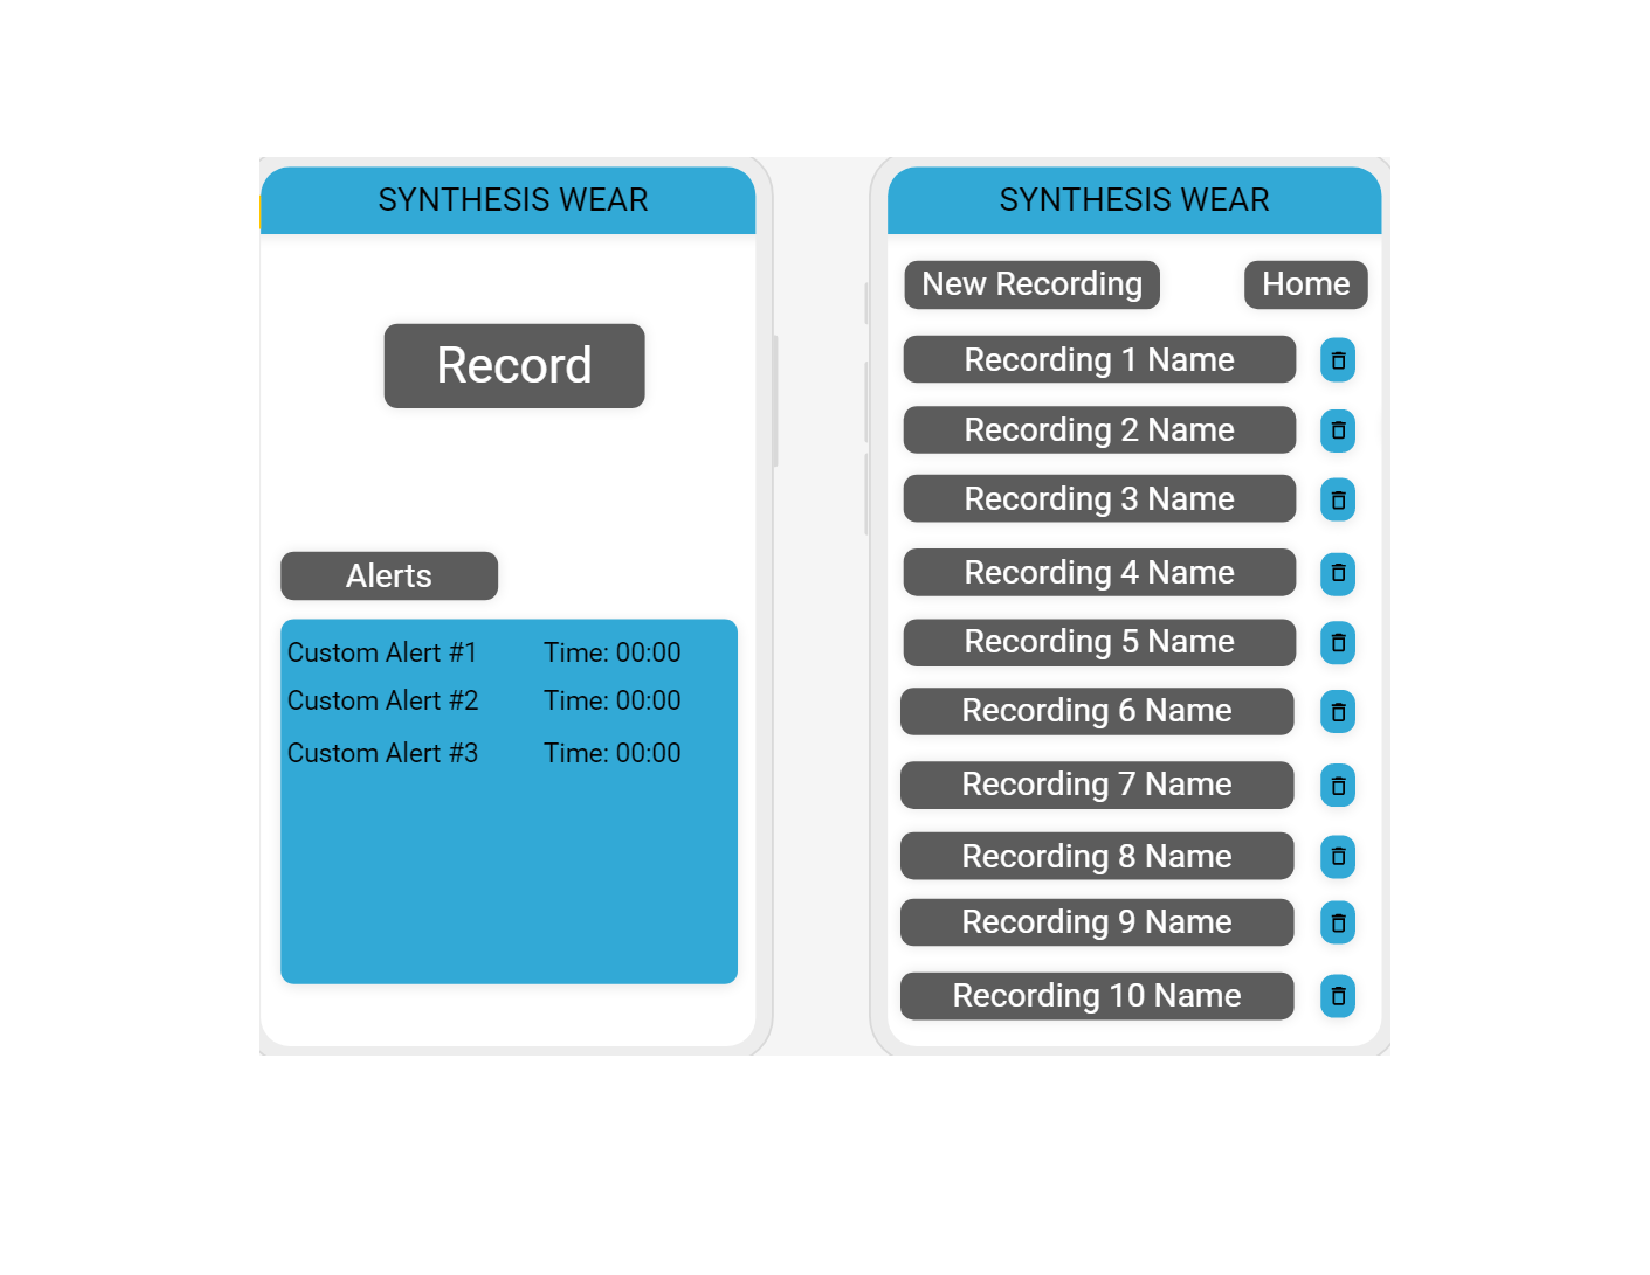
\includegraphics[clip,trim= 0cm 5cm 0cm 2cm,width=\textwidth,height=\textheight,keepaspectratio]{UserInterface.pdf}};
  \draw[red,ultra thick] (image.south east) -- (image.north west);
  \draw[red,ultra thick] (image.north east) -- (image.south west);
  \draw[red,ultra thick] (image.south west) rectangle (image.north east);
\end{tikzpicture}
\begin{center}
  \begin{tabular}{c c}
  \sout{Record} & \sout{Allows users to record new audio to be stored} \\
  \sout{Alters} & \sout{Notifies user of which alter and the timing} \\
  \sout{New Recording} & \sout{Alternative button to change a existing recording} \\
  \sout{Recording Name} & \sout{Name of stored recording} \\
  \sout{Delete} & \sout{Deletion of stored recording} \\
  \sout{Home} & \sout{To go back to main screen} \\
  \end{tabular}
\end{center}

\begin{figure}[H]
  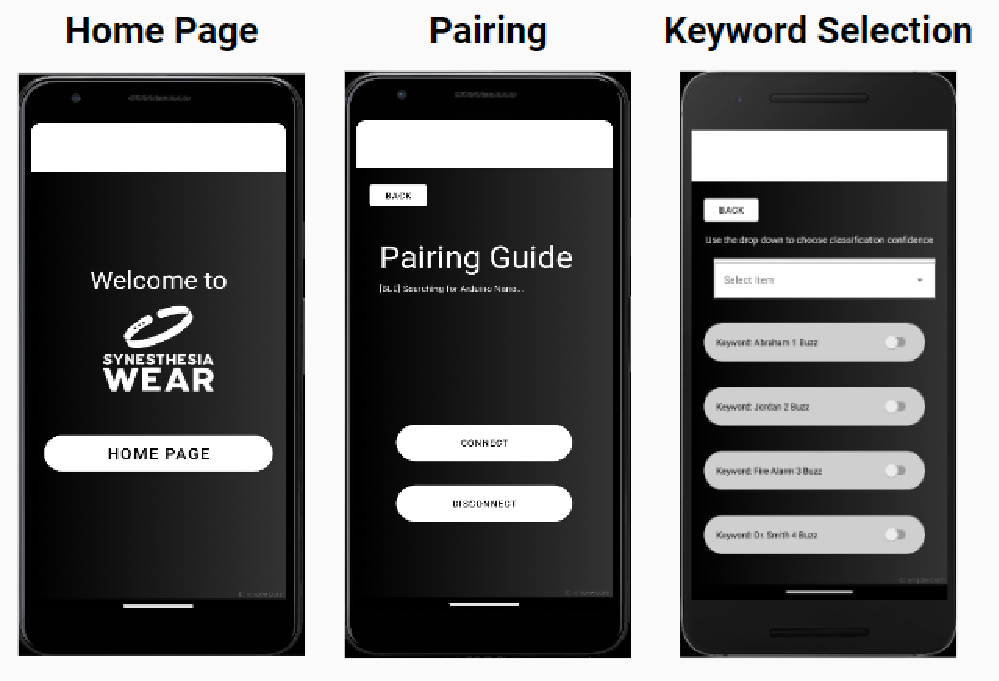
\includegraphics[clip,width=\textwidth,height=\textheight,keepaspectratio]{UserInterface2.pdf}
  \caption{User Interface Mobile}
  \label{User Interface} 
\end{figure}
\begin{center}
  \begin{tabular}{l p{0.8\linewidth}}
  \textcolor{red}{Home Page} & \textcolor{red}{Button that transitions to other features of the app}  \\
  \textcolor{red}{Connect/Disconnect} & \textcolor{red}{Buttons that enable or disable the connection between app and hardware}  \\
  \textcolor{red}{Back} & \textcolor{red}{Button that reverts the current page to the previous page}  \\
  \textcolor{red}{Select Item} & \textcolor{red}{Drop down menu that provides a list of numbers for the minimum confidence level that the sound classification must adhere to}  \\
  \textcolor{red}{Keyword} & \textcolor{red}{Keywords that are toggled on/off to enable/disable them in the sound classification of the device}  \\
\end{tabular}
\end{center}
\newpage

\section{Design of Mechanical Hardware}
\sout{For our project there is limited mechanical hardware required. Most of the components are electrical componets. Regardless the non-electrical componets required are.}
\textcolor{red}{For our project, most of the components are electrical components where there is some mechanical hardware required. With this in mind, the necessary non-electrical components are:}
\begin{table}[H]
\centering
\caption{List of non-electrical components required}
\begin{tabular}{lllll}
S.No & Component        & Material & Link              & Cost  \\ \hline
1    & Base enclosure   & PLA      & In house          & 5     \\
2    & Base lid         & PLA      & In house          & 3     \\
3    & 20mm Watch strap & Silicon  & shorturl.at/hEFM1 & 16.99 \\
4    & Super glue       & Glue     & shorturl.at/CFG09 & 6.27 
\end{tabular}
\label{tab:my-table}
\end{table}

\subsection{Base Enclosure}
This is \textcolor{red}{the} main housing for all the electrical components. It houses the microcontroller, the vibration motor, the battery and the battery management system. It will be 3D printed using PLA as the Material. This housing also provides the additional ability to attach 20 mm watch straps to it.
Below are two isometric \textcolor{red}{views} of the Base enclosure. 
\begin{figure}[H]
  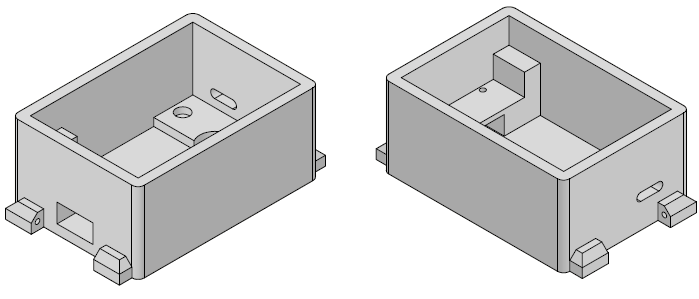
\includegraphics[width=\textwidth,height=\textheight,keepaspectratio]{Base_ISO.png}
  \caption{Enclosure isometric figures}
  \label{EnclosureISO} 
\end{figure}
\noindent There are specifc slots for all the major \sout{componets} \textcolor{red}{components} like the microcontroller, vibration motor, battery, etc. There are also cutouts for the usb C charging port for the battery and a cutout for the battery enable switch. For a detailed drawing refer to the \hyperref[appendix:hardware:enclosureDWG]{Appendix}. The drawing does not show all the dimensions for clarity reasons but it does show the outer dimensions. An \sout{explosed} \textcolor{red}{exploded} diagram with all the components will be shown later in the section. 
 
\subsection{Enclosure lid}
This is the lid for the enclosure that was shown above. It will also be made in house on a 3D printer with PLA plastic. It will be secured to the enclosure using super glue once proper functioning of all the components is achieved. 
Below is an isometric \sout{diagram for} \textcolor{red}{view of} the lid.\\
\begin{figure}[H]
  \vspace*{-0.5cm}
  \centering
  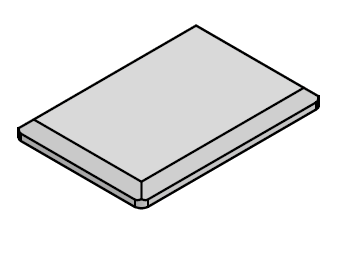
\includegraphics[width=\textwidth,height=\textheight/2,keepaspectratio]{Lid_ISO.png}
  \vspace*{-2cm}
  \caption{lid isometric figure}
  \label{Lid ISO} 
\end{figure}
\noindent For a detailed drawing refer to the \hyperref[appendix:hardware:lidDWG]{Appendix}. The drawing does not show all the dimensions for clarity reasons but it does show the outer dimensions.

\subsection{Watch straps}
A pair of standard 20 mm watch straps will be aquired from external sources. For the material, we have selected silicone rubber as it would be the most durable along with it being cost effective. It is estimated to cost 16.99 CAD. This will attach to the base enclosure using standard 1.5 mm spring jumper lugs that come included with the watch straps. This should enable the user to have the device mounted on \sout{the user} \textcolor{red}{their wrist} without the user having to carry it in \sout{the user's hand} \textcolor{red}{their hands}.

\subsection{Super glue}
Super glue will be used to secure most of the componets in place either directly or indirectly. For the lid it can be directly attached using super glue. However\textcolor{red}{,} for the PCBs they have to be attached using plastic dowels with a lid and super glue. There are already holes placed in the enlosure for these \sout{fastners} \textcolor{red}{fasteners}. \sout{The use of threaded fasterners was} \textcolor{red}{Threaded fasteners were} not used due to the difficulty of adding threads \sout{accuratly} \textcolor{red}{accurately} to the plastic enclosure. The disadvange of using the super glue along with the plastic dowels is that once secured\textcolor{red}{,} they are permenent.   

\subsection{Complete assembly}
\sout{The entire hardware is enclosed} \textcolor{red}{All of the hardware is contained} between the enslosure and the lid. An isometric \textcolor{red}{view} of the complete assembly is shown below. \\
\begin{figure}[H]
  \vspace*{-0.75cm}
  \centering
  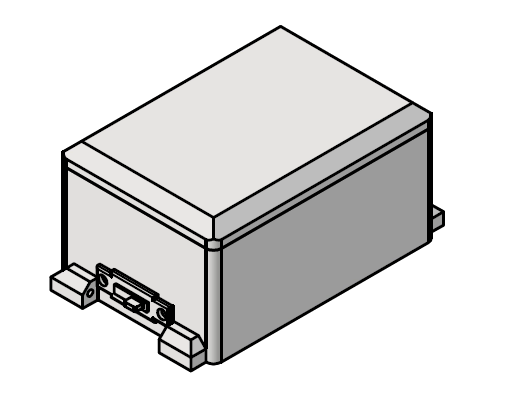
\includegraphics[width=\textwidth,height=\textheight/2,keepaspectratio]{Assembly_ISO.png}
  \caption{Assembly isometric figure}
  \label{Assembly ISO} 
\end{figure}
\noindent The exploded assembly is shown below. \\
\begin{figure}[H]
  \centering
  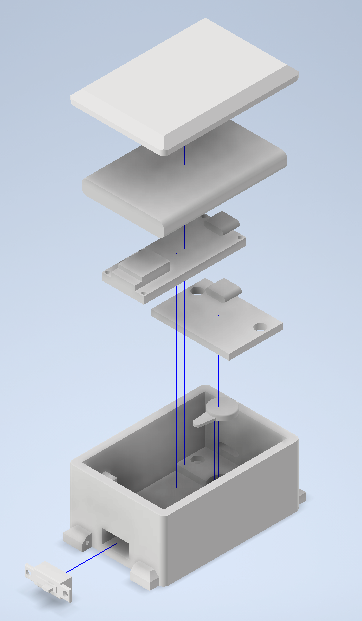
\includegraphics[width=\textwidth,height=\textheight/2,keepaspectratio]{Exploded_view.png}
  \caption{Exploded view of the assembly}
  \label{Exploded} 
\end{figure}
\noindent For a detailed drawing refer to the \hyperref[appendix:hardware:assembly]{Appendix}. The drawing does not show all the dimensions for clarity reasons but it does show the outer dimensions.

\newpage

\section{Design of Electrical Components}
A list of electrical components required is listed below. \\
\begin{table}[H]
  \scriptsize	
  \vspace*{-0.5cm}
  \caption{Electrical Components List}
  \vspace*{-0.5cm}
  \begin{center}
  \begin{tabular}{| p{0.25\textwidth} | p{0.08\textwidth}  | p{0.10\textwidth} | p{0.15\textwidth} | p{0.30\textwidth} |}
   \hline
  \textbf{Component} & \textbf{Amount} & \textbf{Cost \quad \quad (in CAD\$)} & \textbf{Dimensions} & \textbf{Link} \\ \hline

  Arduino Nano 33 BLE	& 2 & 80 & 48 * 18 & 	\url{https://www.amazon.ca/Arduino-Nano-33-BLE-Sense/dp/B07WV5GF17} \\ \hline
  Lithium-Ion Polymer (LiPo) Battery (3.7V 1000mAh)	& 1	& 10 & 50*32*5 & 	\url{https://www.canadarobotix.com/products/588} \\ \hline
  0.1 microfarad capacitor	& 2 &	1.11 &	5*3	& \url{https://rb.gy/vyewya} \\ \hline
  Resistor 1000 ohm	& 1	& NA &	5*3 &	At home \\ \hline
  Resistor 20 ohm &	1 &	NA &	5*3 &	At home \\ \hline
  Vibration motor &	5 &	10 &	10*2 &	\url{https://www.amazon.ca/dp/B089NTLLWB?ref_=cm_sw_r_apin_dp_YEQ7CS0SNQV7HKHZZVFD} \\ \hline
  Transistor NPN - PN2222 &	1 &	NA &	5*3 &	At home \\ \hline
  Diode - IN4007 &	1 & 	NA &	5*3 &	At home \\ \hline
  Power Management module & 2 &	17.5 &	35*22 &	\url{https://www.digikey.com/en/products/detail/sparkfun-electronics/PRT-14411/1568-1723-ND/7725301} \\ \hline
  E-Switch Slide switch & 1 &	1.04 &	19*6*5 &	\url{https://www.shorturl.at/jMN791} \\ \hline
  \end{tabular}
  \end{center}
  \hspace*{-1cm}
  \end{table}

\subsection{Complete electrical layout}
The entire electrical system can be split into 3 parts
\begin{itemize}
  \item Microcontroller
  \item Battery System 
  \item Vibration motor and related electrical components
\end{itemize}

\noindent The complete layout of the electrical \sout{componets} \textcolor{red}{components} are shown below, explanations for the components will come in the later sections.
\begin{figure}[H]
\centering
  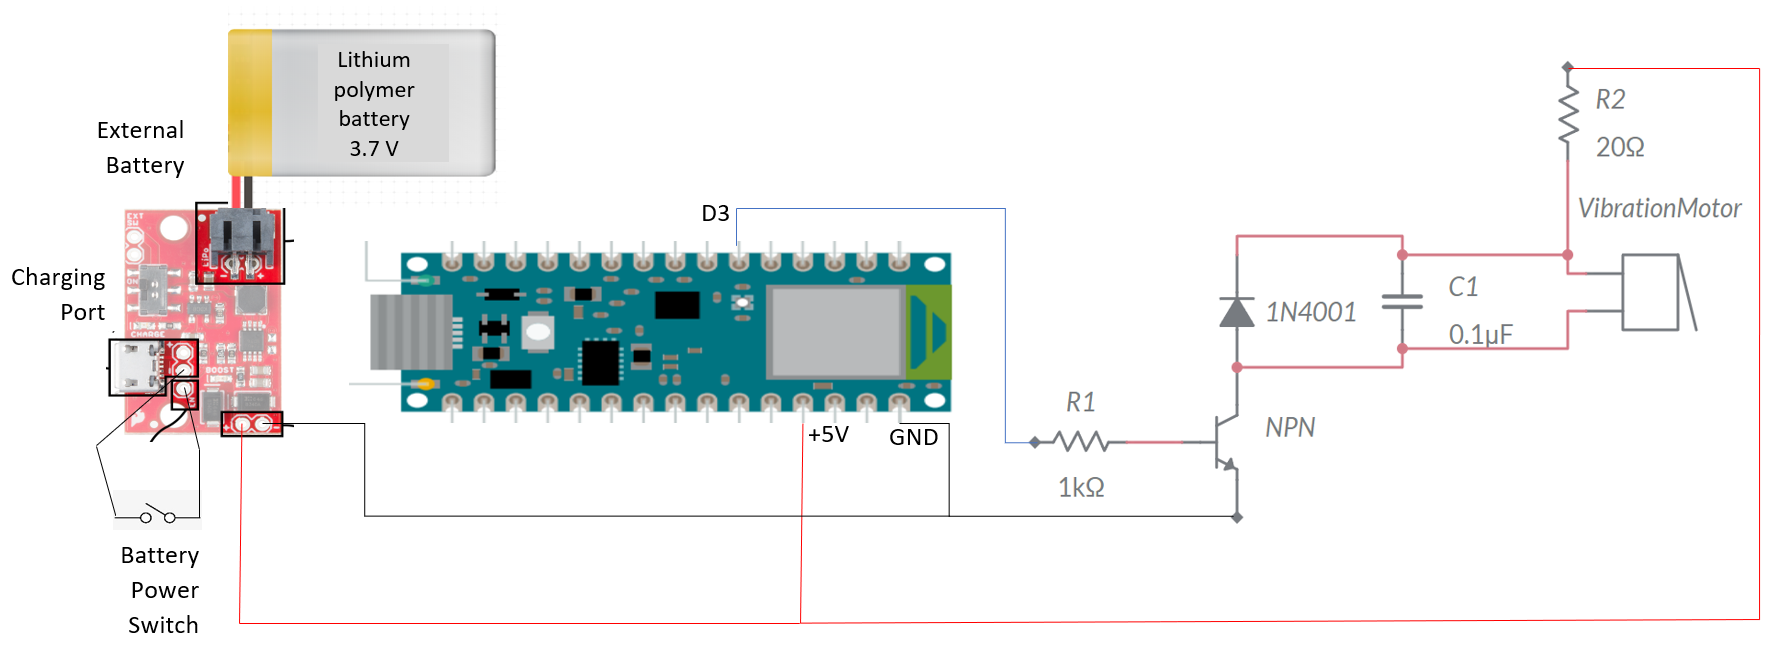
\includegraphics[width=\textwidth,height=\textheight,keepaspectratio]{Schematic.png}
  \caption{Complete electrical schematic}
  \label{schematic} 
\end{figure}

\subsection{Microcontroller}
The microcontroller is responsible for most of the the application of the device. It will handle audio dectection, audio processing classification and bluetooth communication. The microcontroller selected is an Arduino nano 33 BLE. This was selected as it is relatively compact with bluetooth and microphone already built into the device. It will be supplied by an external power source of 5V connected directly to the +5V and GND of the Arduino. A digital pin (D3) will be used to control the vibration motor. Below is the schematic of the microcontroller.
 \begin{figure}[H]
\centering
  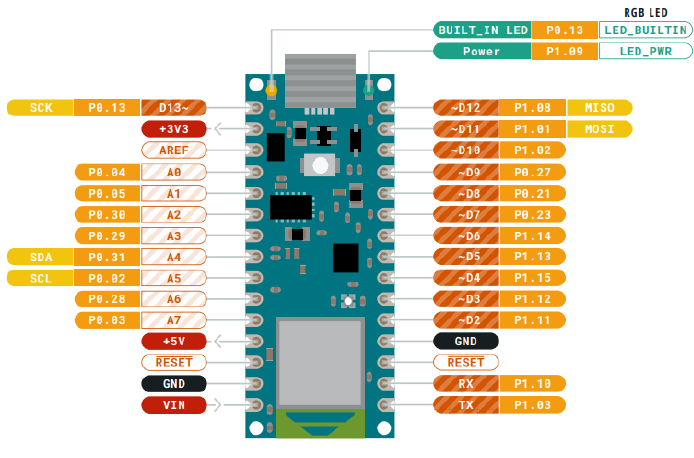
\includegraphics[width=\textwidth,height=\textheight,keepaspectratio]{NanoSchematic.png}
  \caption{Arduino schematic}
  \label{Nanoschematic} 
\end{figure}

\subsection{Battery/Power System}
The Arduino will be powered by a 5 Volt battery system that can supply up to 1A of current. This should be well within the operating region of the Arduino. The battery system consists of a 3.7 Volt 1000mAh  LiPo battery, a SparkFun LiPo Charger/Booster and a small slide switch. The 3.7 Volt LiPo was selected as it is small enough to fit within the design and has enough capacity for a day of usage. The SparkFun LiPo Charger/Booster is used to boost the voltage from 3.7 to 5 Volts \sout{as} \textcolor{red}{since} that is required by the Arduino. It also provides the additional \sout{benifit} \textcolor{red}{benefit} of protecting the battery from high currents. The battery can also be charged using the usb C port on the SparkFun LiPo Charger/Booster. A switch will be soldered on to the enable pin of the charger/booster\sout{, this will} \textcolor{red}{to} provide a way to isolate the battery from the microcontroller and \sout{can} act like a reset switch. The Ardunio power input will have to be soldered onto the booster output connection. The battery can either be attached using a JST connector or can be soldered on. Below is the schematic for the battery system.   
 \begin{figure}[H]
\centering
  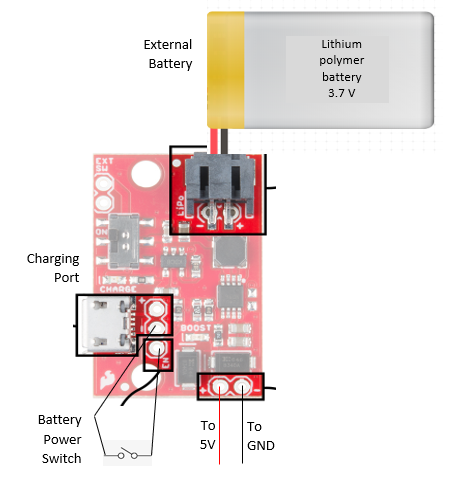
\includegraphics[width=\textwidth,height=\textheight/2,keepaspectratio]{BatterySchematic.png}
  \caption{Battery system schematic}
  \label{batteryschematic} 
\end{figure}

\subsection{Vibration motor and related components}
The user will be alerted using the vibration motor that is recessed into the enclosure. The vibration motor needs a significant amount of current that the digital output pin cannot supply. Hence the digital pin is just used as an enable pin and the current for the motor is drawn from the 5V pin. To achieve this\textcolor{red}{,} an NPN transistor (PN2222) is used as a switch with the digital output pin being its \sout{enable} \textcolor{red}{enabler}. Resistors are also used to limit the current draw of the motor. A capacitor is used to protect from high current \sout{impluses} \textcolor{red}{impulses} and a diode is used to protect the Arduino from backflow in case the motor stalls. The schematic for the circuit is given below. The components will be soldered together with \sout{little} \textcolor{red}{some} wires \sout{and} \textcolor{red}{while} heat shrink will be used over them to prevent shorts. The \sout{componets} \textcolor{red}{components} will be placed next to \textcolor{red}{the} vibration motor \textcolor{red}{which is} right below the battery booster board. 

 \begin{figure}[H]
\centering
  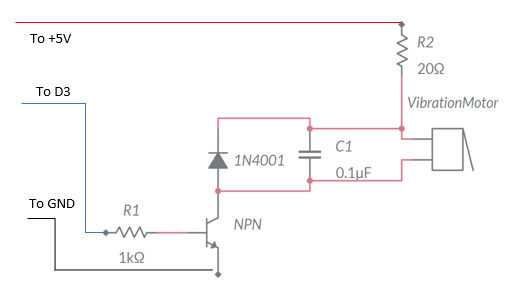
\includegraphics[width=\textwidth,height=\textheight,keepaspectratio]{MotorSchematic.png}
  \caption{Vibration motor schematic}
  \label{Vibration motor schematic} 
\end{figure}

\section{Design of Communication Protocols}
In regards to communication protocols, the only relevant aspect of Synesthesia Wear would revolve around the bluetooth functionality of the system.
As stated in \autoref{table:Connections Table}, the microcontroller used for Synesthesia Wear has a built-in bluetooth module that was purchased for the purposes of reducing product dimensions as much as possible.
With this in mind, the system was set up so that this same bluetooth module would be able to connect to the Synesthesia Wear application on the user's device and thus be able to communicate between each other.

\begin{figure}[H]
  \vspace*{-2cm}
  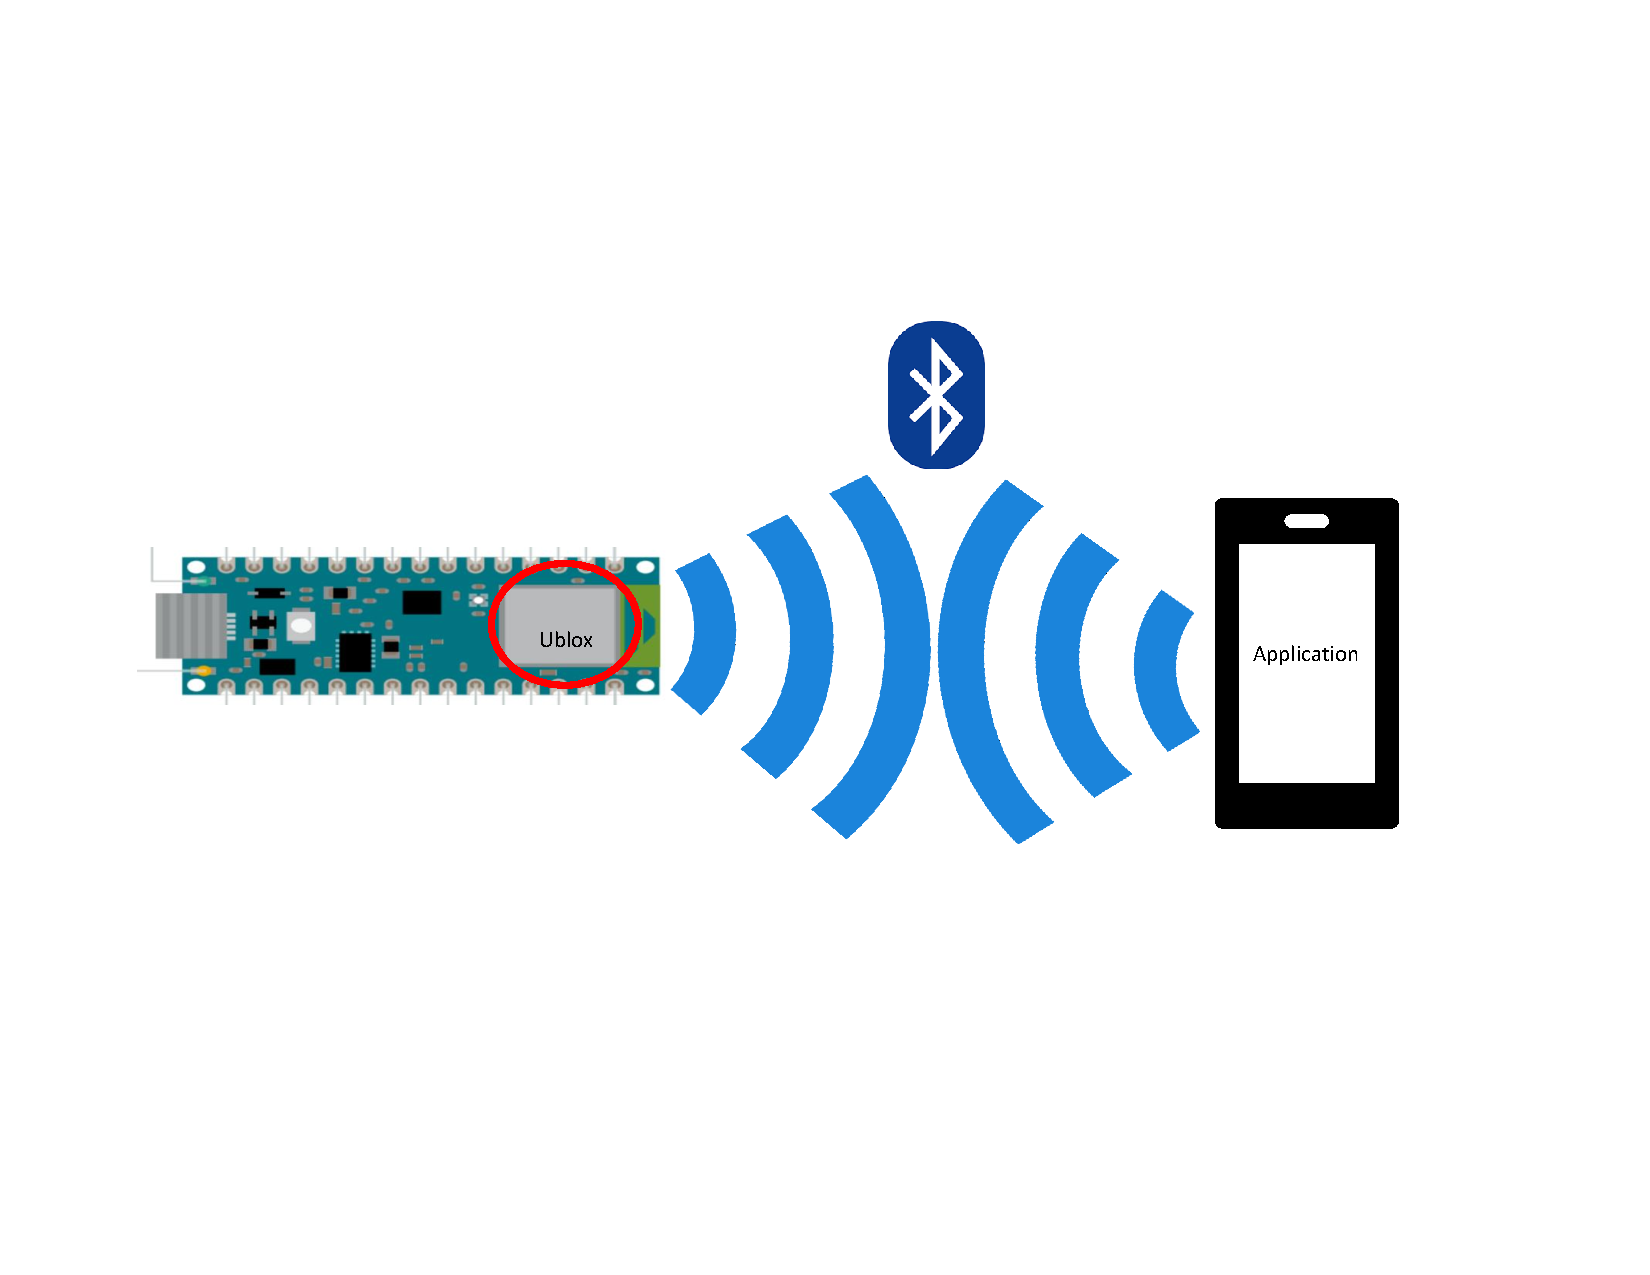
\includegraphics[width=\textwidth,height=\textheight,keepaspectratio]{BluetoothConnection.pdf}
  \vspace*{-4cm}
  \caption{Bluetooth Connection between device and microcontroller}
  \label{Bluetooth Connection} 
\end{figure}

\section{Timeline}
\begin{tikzpicture}
  \node[inner sep=0] (image) at (0,0) {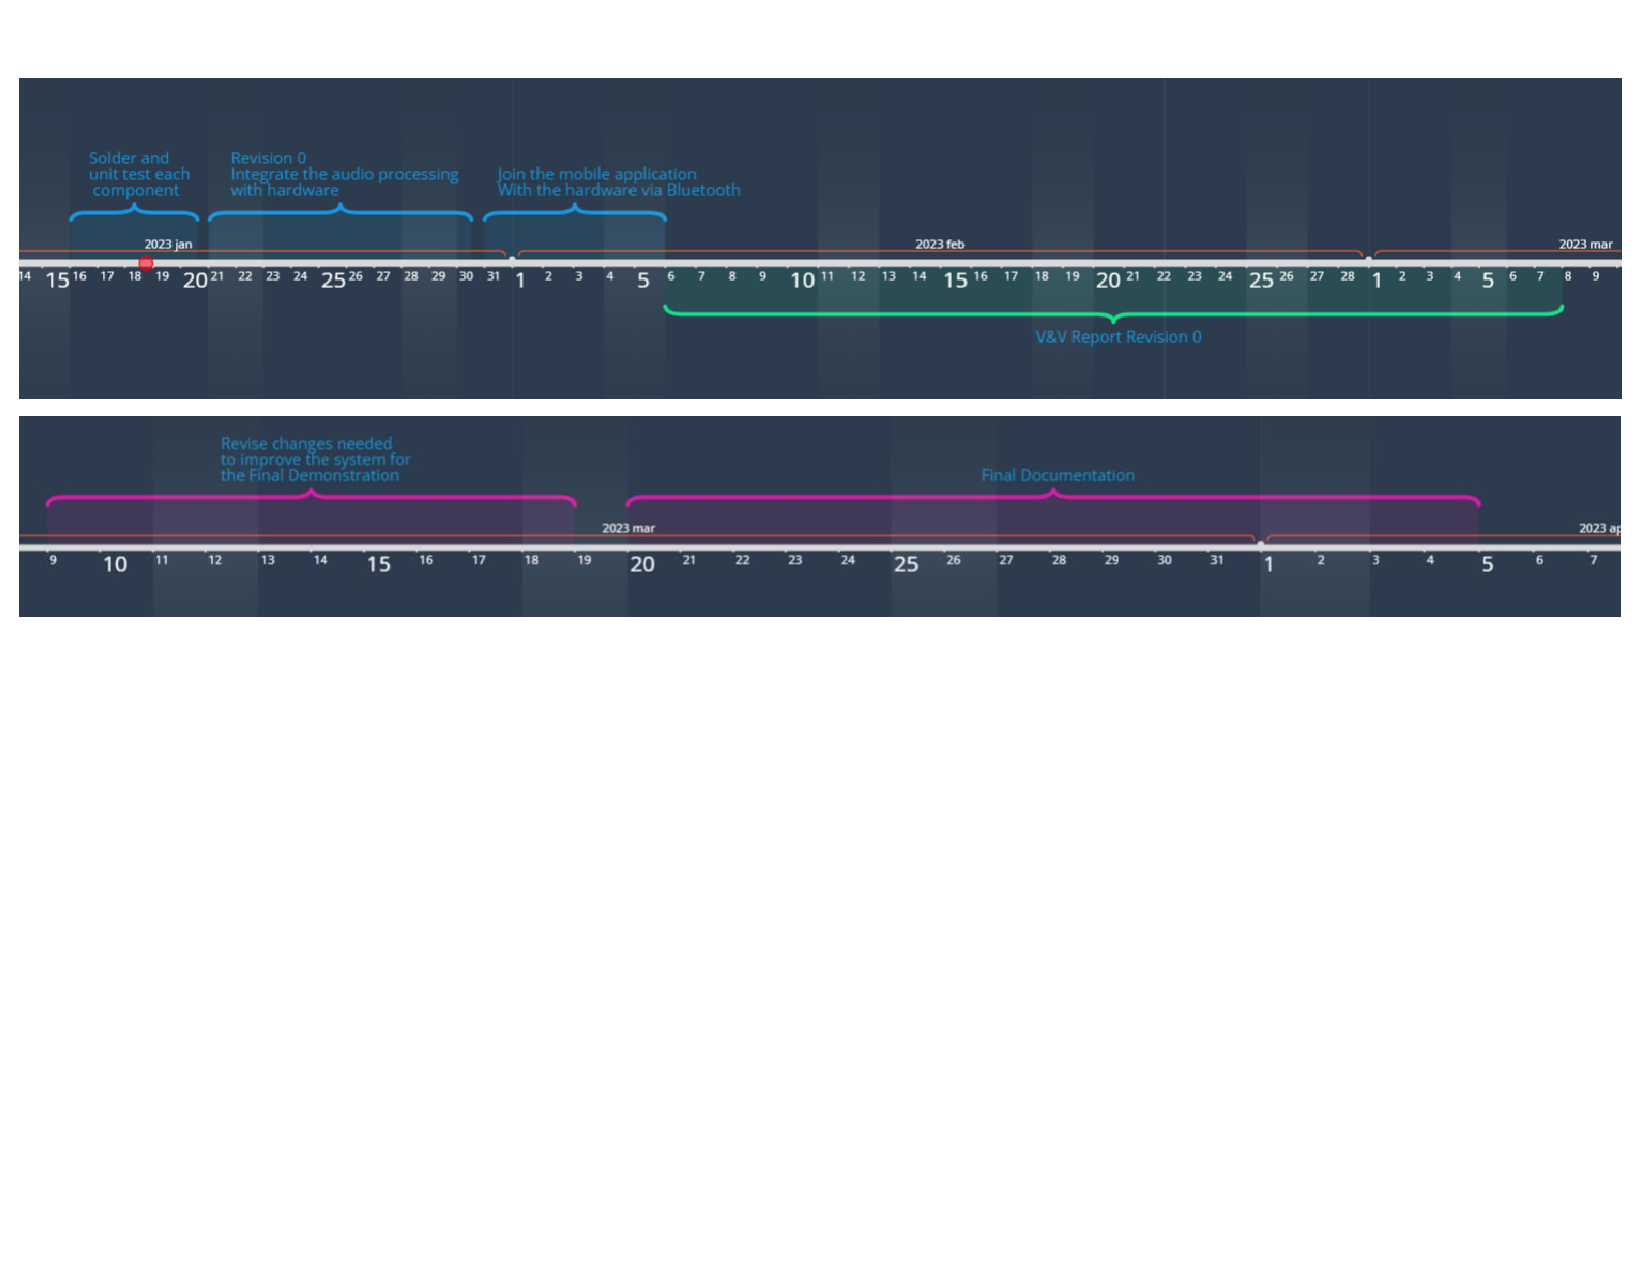
\includegraphics[clip,trim= 1cm 11.5cm 1cm 1.5cm,width=\textwidth,height=\textheight,keepaspectratio]{Timeline.pdf}};
  \draw[red,ultra thick] (image.south east) -- (image.north west);
  \draw[red,ultra thick] (image.north east) -- (image.south west);
  \draw[red,ultra thick] (image.south west) rectangle (image.north east);
\end{tikzpicture}

\begin{figure}[H]
  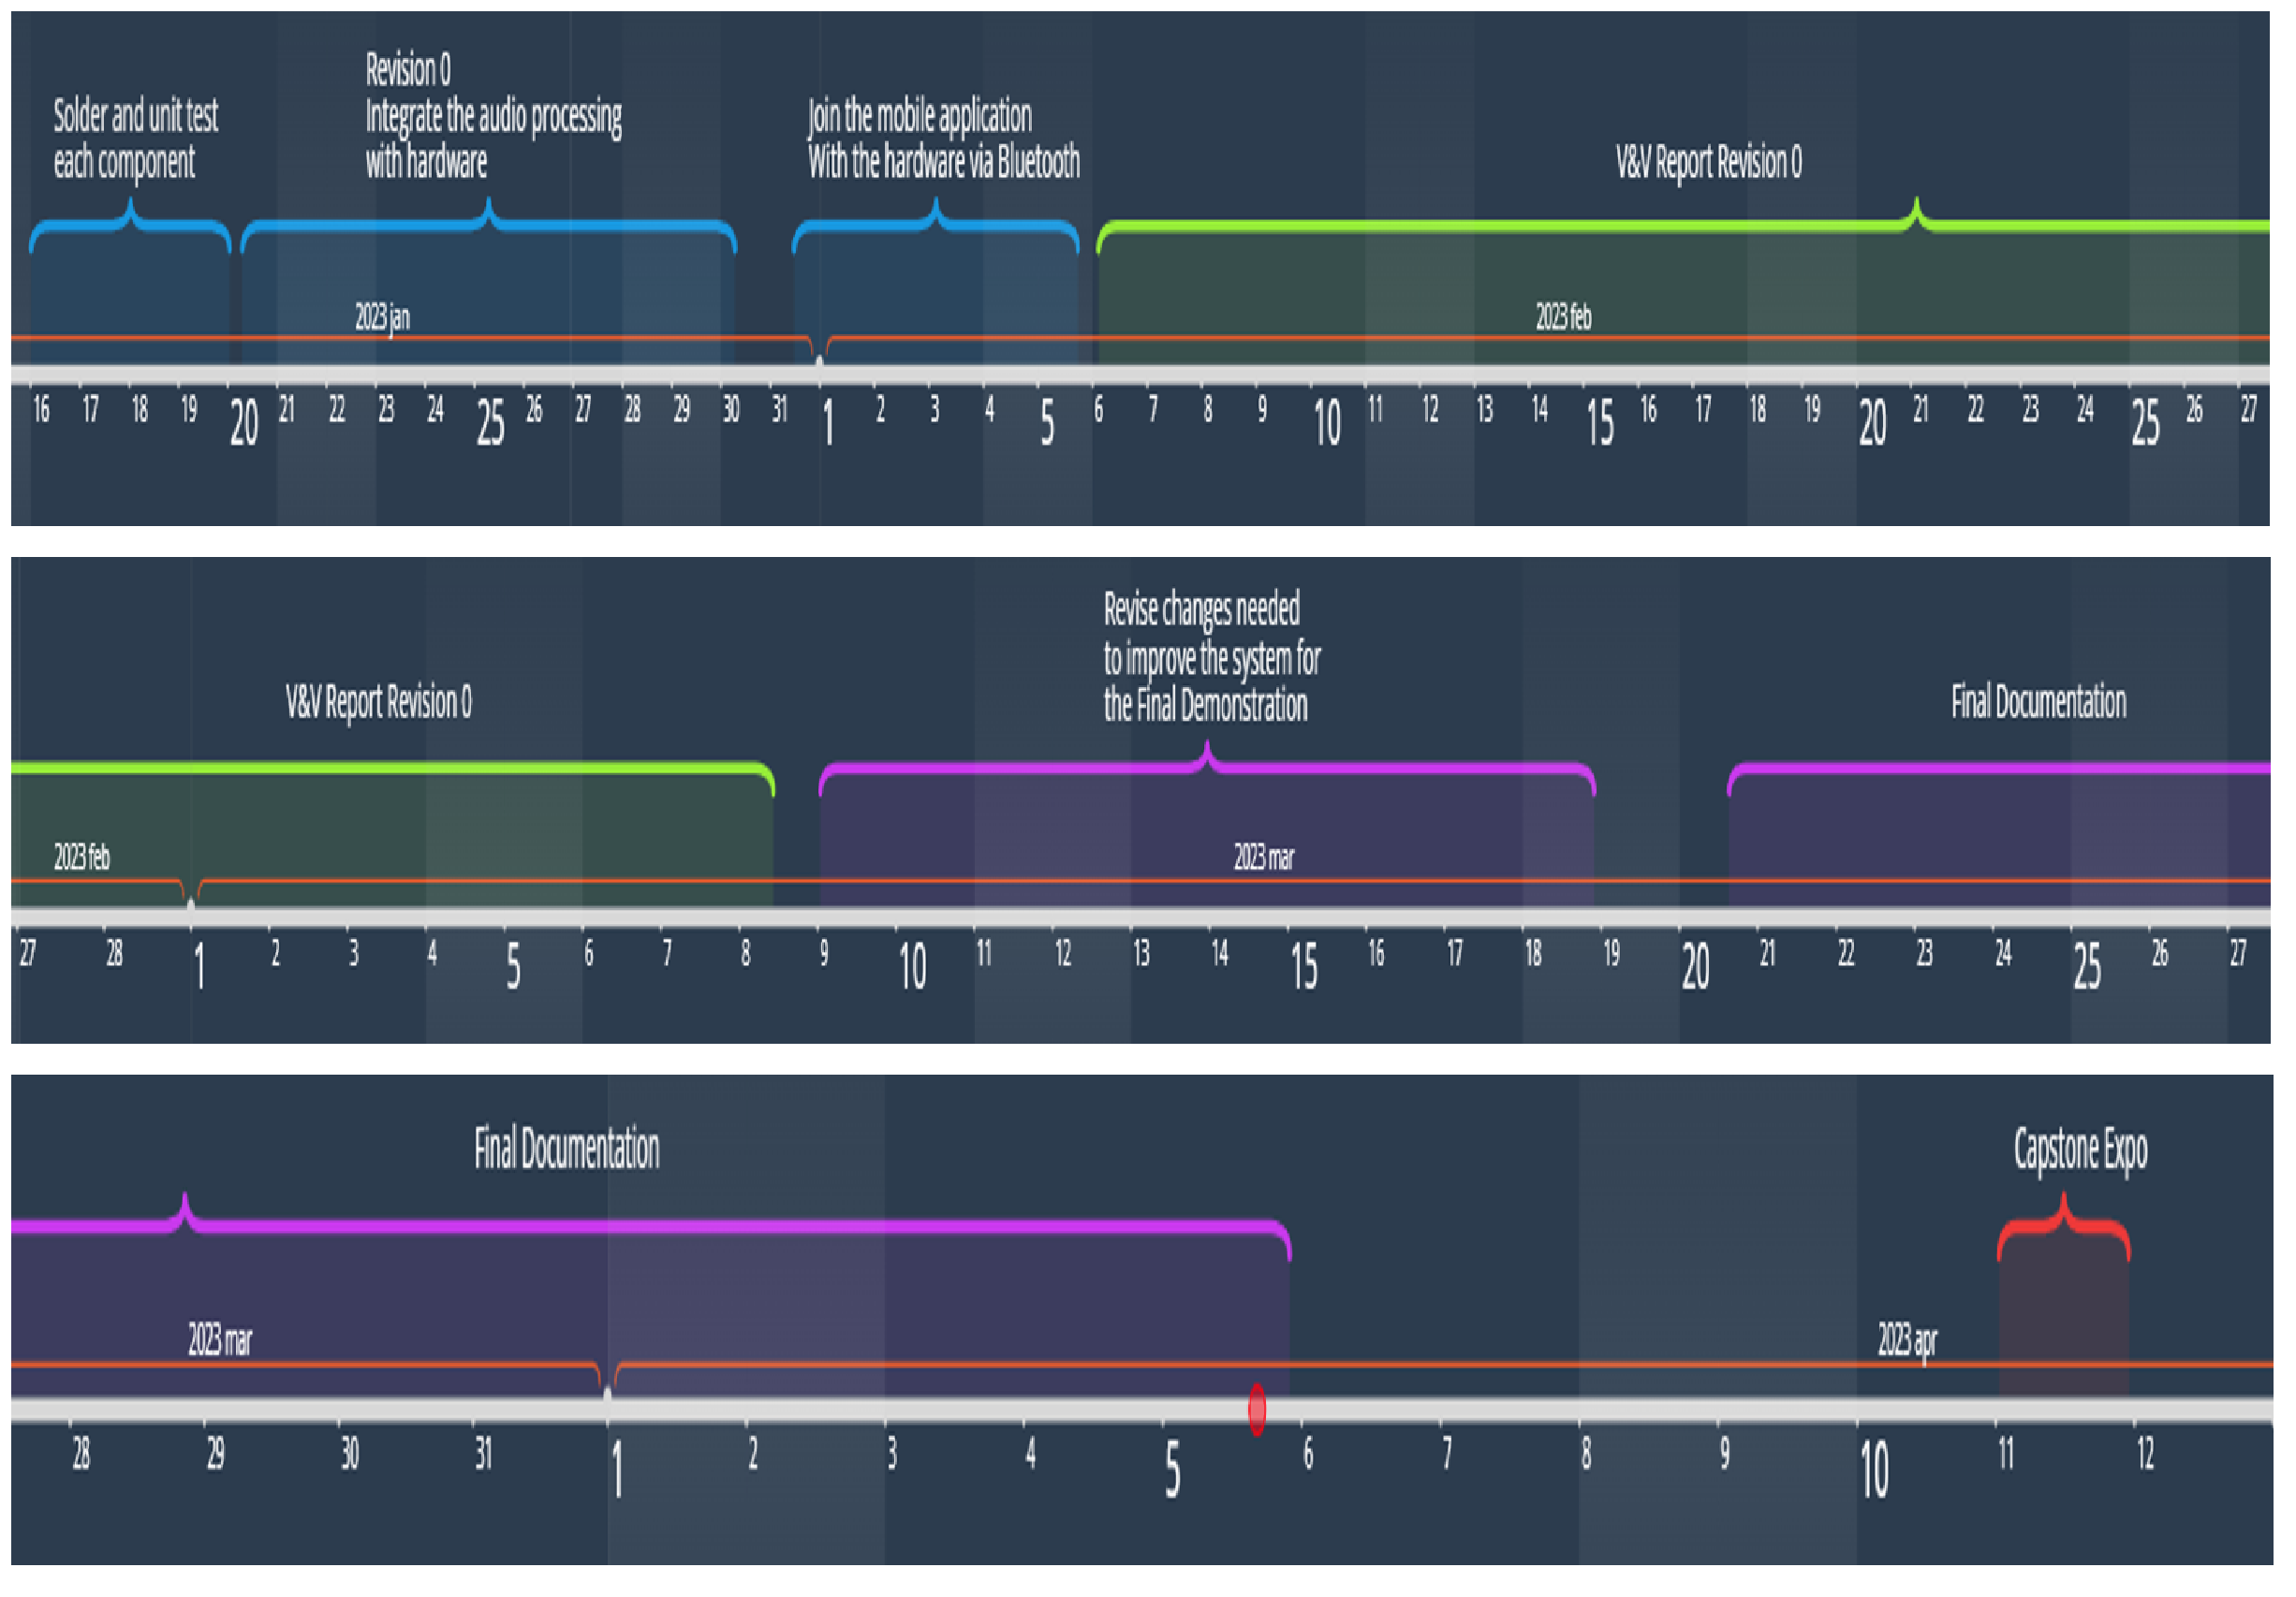
\includegraphics[clip,width=\textwidth,height=\textheight,keepaspectratio]{Timeline2.pdf}
  \caption{Timeline}
  \label{Timeline} 
\end{figure}

\begin{center}
\begin{table}[H]
  \caption{\textcolor{red}{STRONE Member Responsibilities}}
  \centering
  \begin{tabular}{|l|p{0.75\linewidth}|}
  \hline
  \textcolor{red}{Jordan Bierbrier} & \textcolor{red}{Sound classification module development: responsible for getting the machine learning model properly implemented and trained.}  \\
  \hline
  \textcolor{red}{Azriel Gingoyon} & \textcolor{red}{Sound classification module development: responsible for getting desirable sound recognition functionality integrated with the hardware}  \\
  \hline
  \textcolor{red}{Taranjit Lotey} & \textcolor{red}{Mobile App development: responsible for getting the application pages properly designed and implemented.}  \\
  \hline
  \textcolor{red}{Udeep Shah} & \textcolor{red}{Hardware Development: responsible for 3D printing as well as putting all of the hardware together.}  \\
  \hline
  \textcolor{red}{Abraham Taha} & \textcolor{red}{Mobile App Development: responsible for getting the bluetooth connection and application features working.}  \\
  \hline
  \end{tabular}
\end{table}
\end{center}


\subsection{Solder and Unit Testing}
\begin{itemize}
\item Connect and test micro controller with vibrating motor.
\item Use module "Start" as part of Arduino library to test the vibrating motor.
\item Use module "Record" as part of Arduino library to test the microphone.
\end{itemize}



\subsection{Integrate Audio Processing}

Listed in order of high priority:
\begin{itemize}
\item Create module "Bluetooth Connection", establish a successful connection
\item Create module "Output Signal", what will be the output signal for each signal
\item Create module "Sound Classification", \sout{category} \textcolor{red}{categories} of sound produced
\item Create module "Battery Status", indication of low battery status
\item Create module "Microphone", collect the audio recording
\end{itemize}

\subsection{Mobile Application and Hardware Connection}

\begin{itemize}
\item \sout{Create module "Login", create a personalized login} \textcolor{red}{(Design decision was made to remove Authentication/Login aspects of the project)}
\item Create module "Keyword Selection", categorize the recordings
\item \sout{Create module "Profile Module", load the user data}
\item Create module "Bluetooth Communication", communication integrator
\end{itemize}

\newpage{}

\begin{appendices}
  \section{Mechanical Hardware}
  \label{appendix:hardware}
\subsection{Enclosure Drawings}
  \begin{center}
	\label{appendix:hardware:enclosureDWG}
  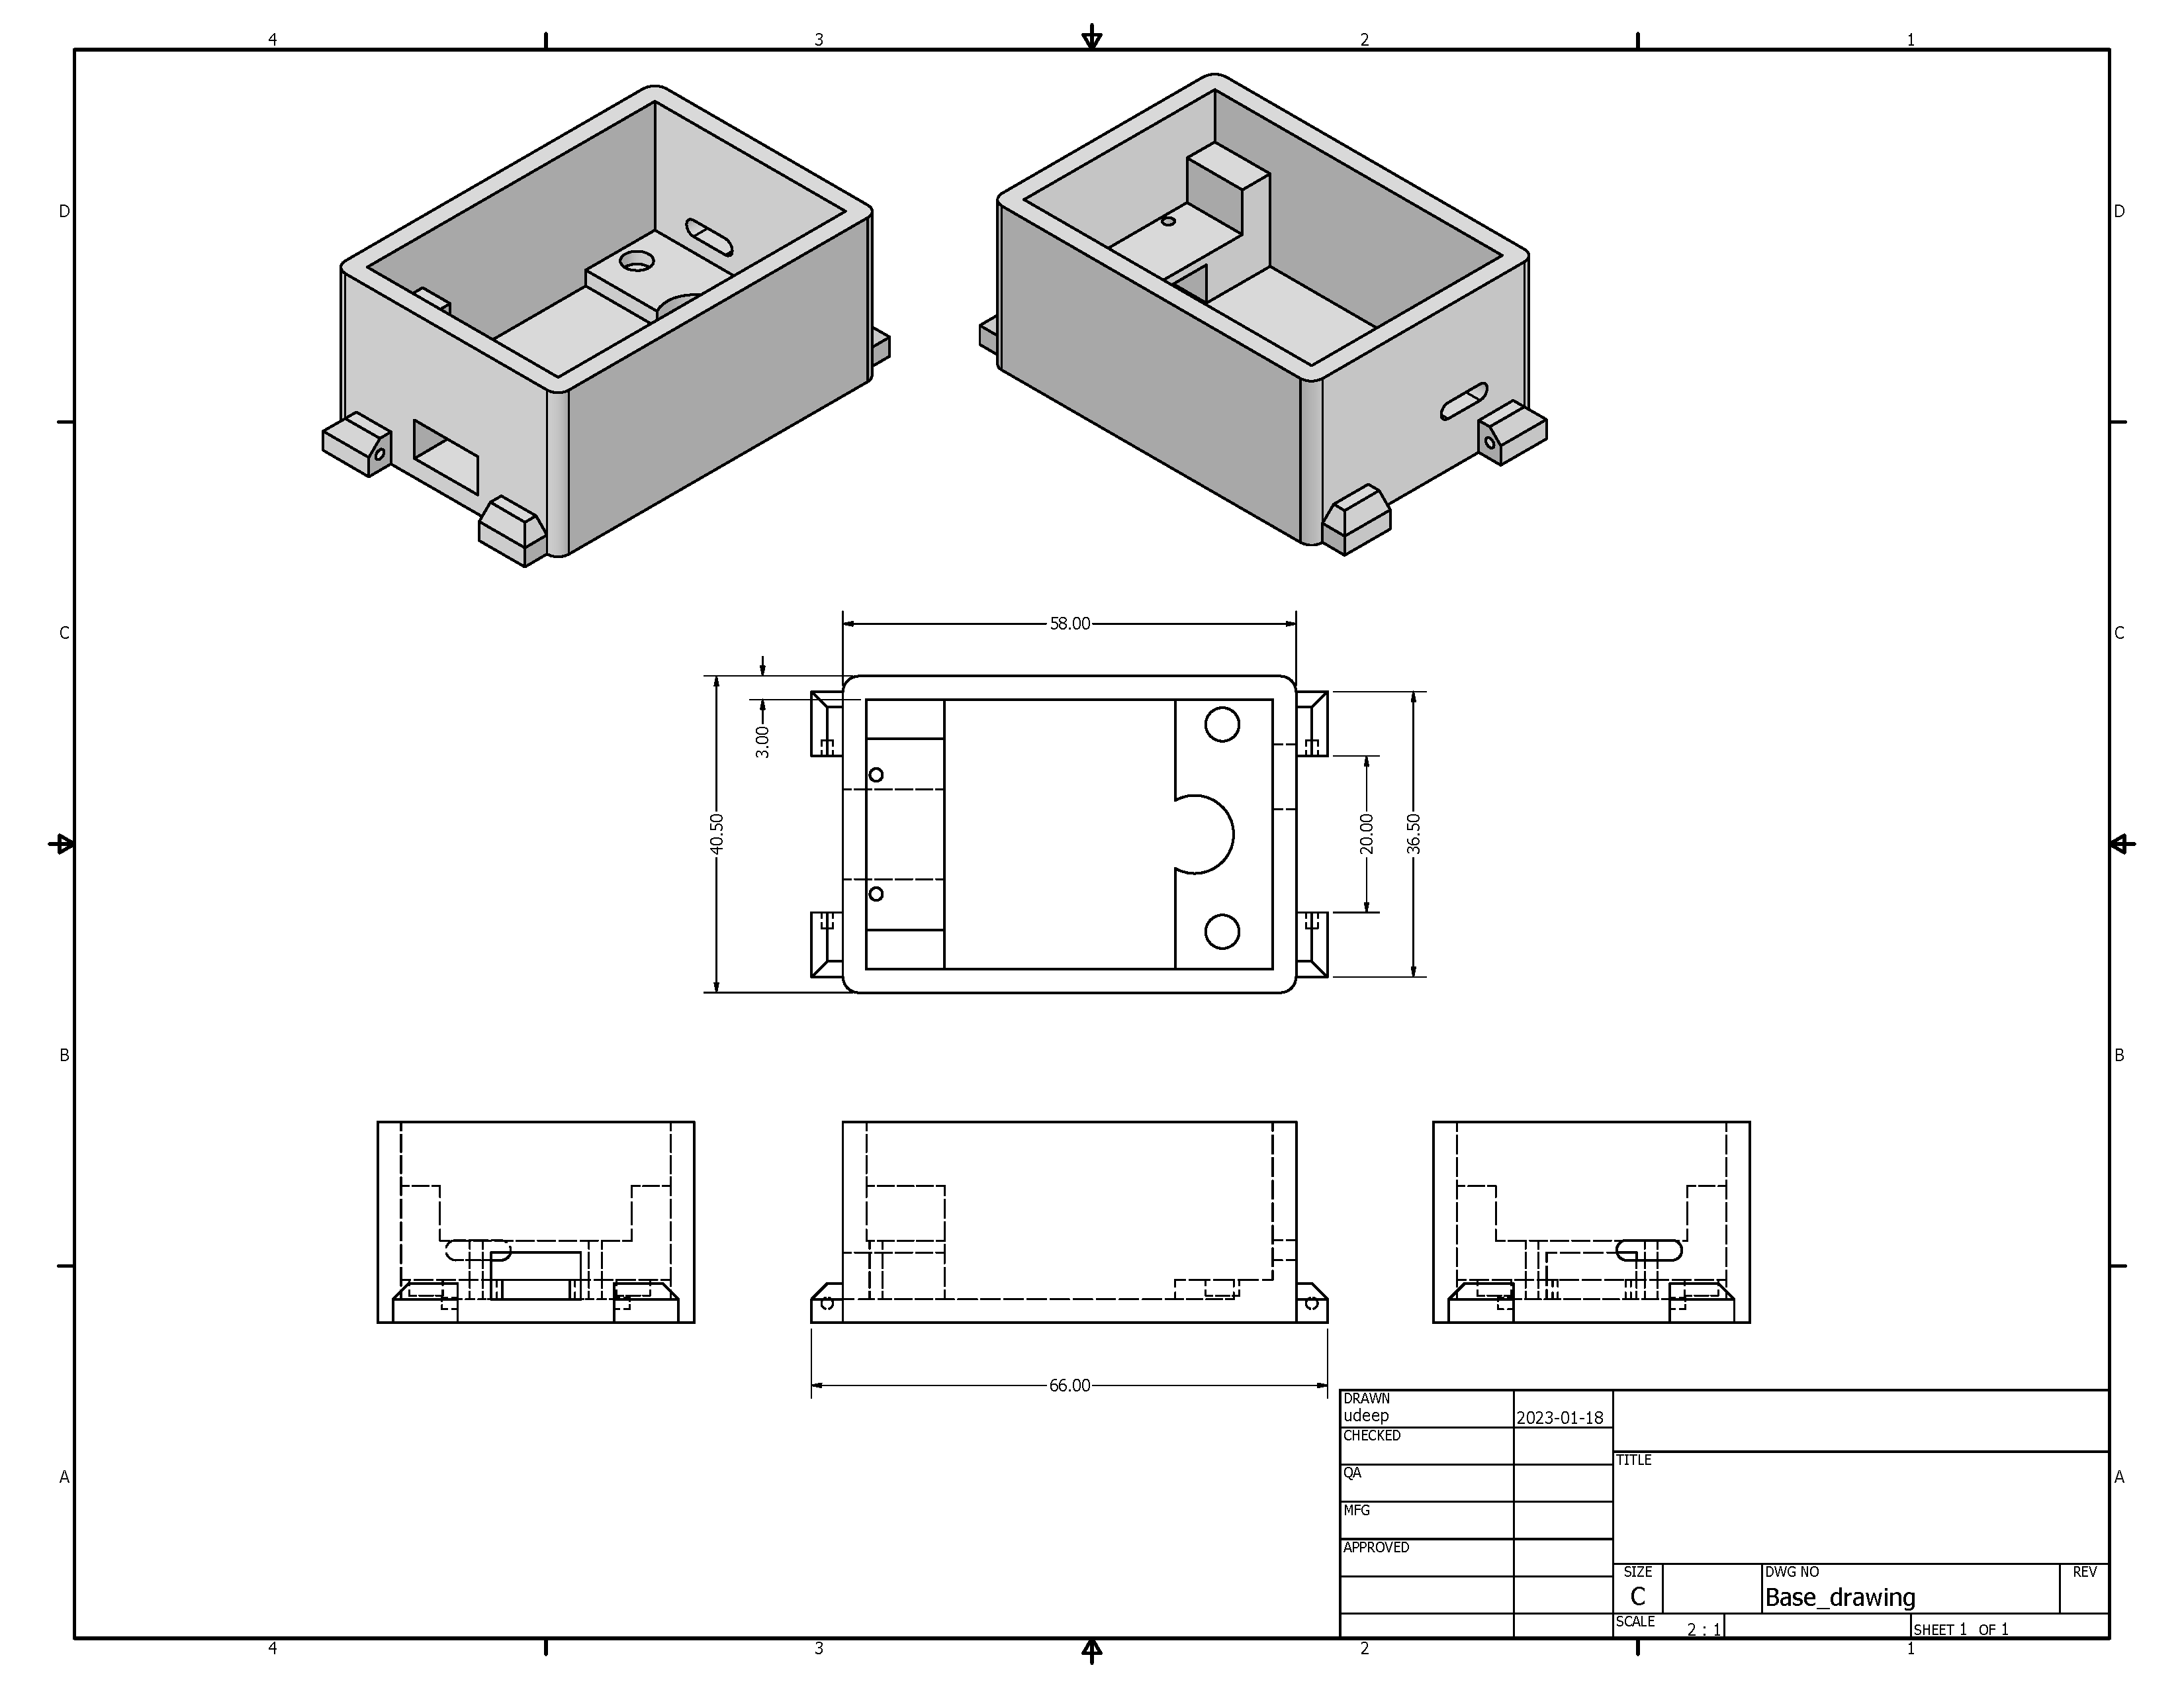
\includegraphics[width=\textwidth,height=\textheight,keepaspectratio]{Base_drawing.pdf}
\end{center}
\subsection{Lid Drawings}
	\label{appendix:hardware:lidDWG}

  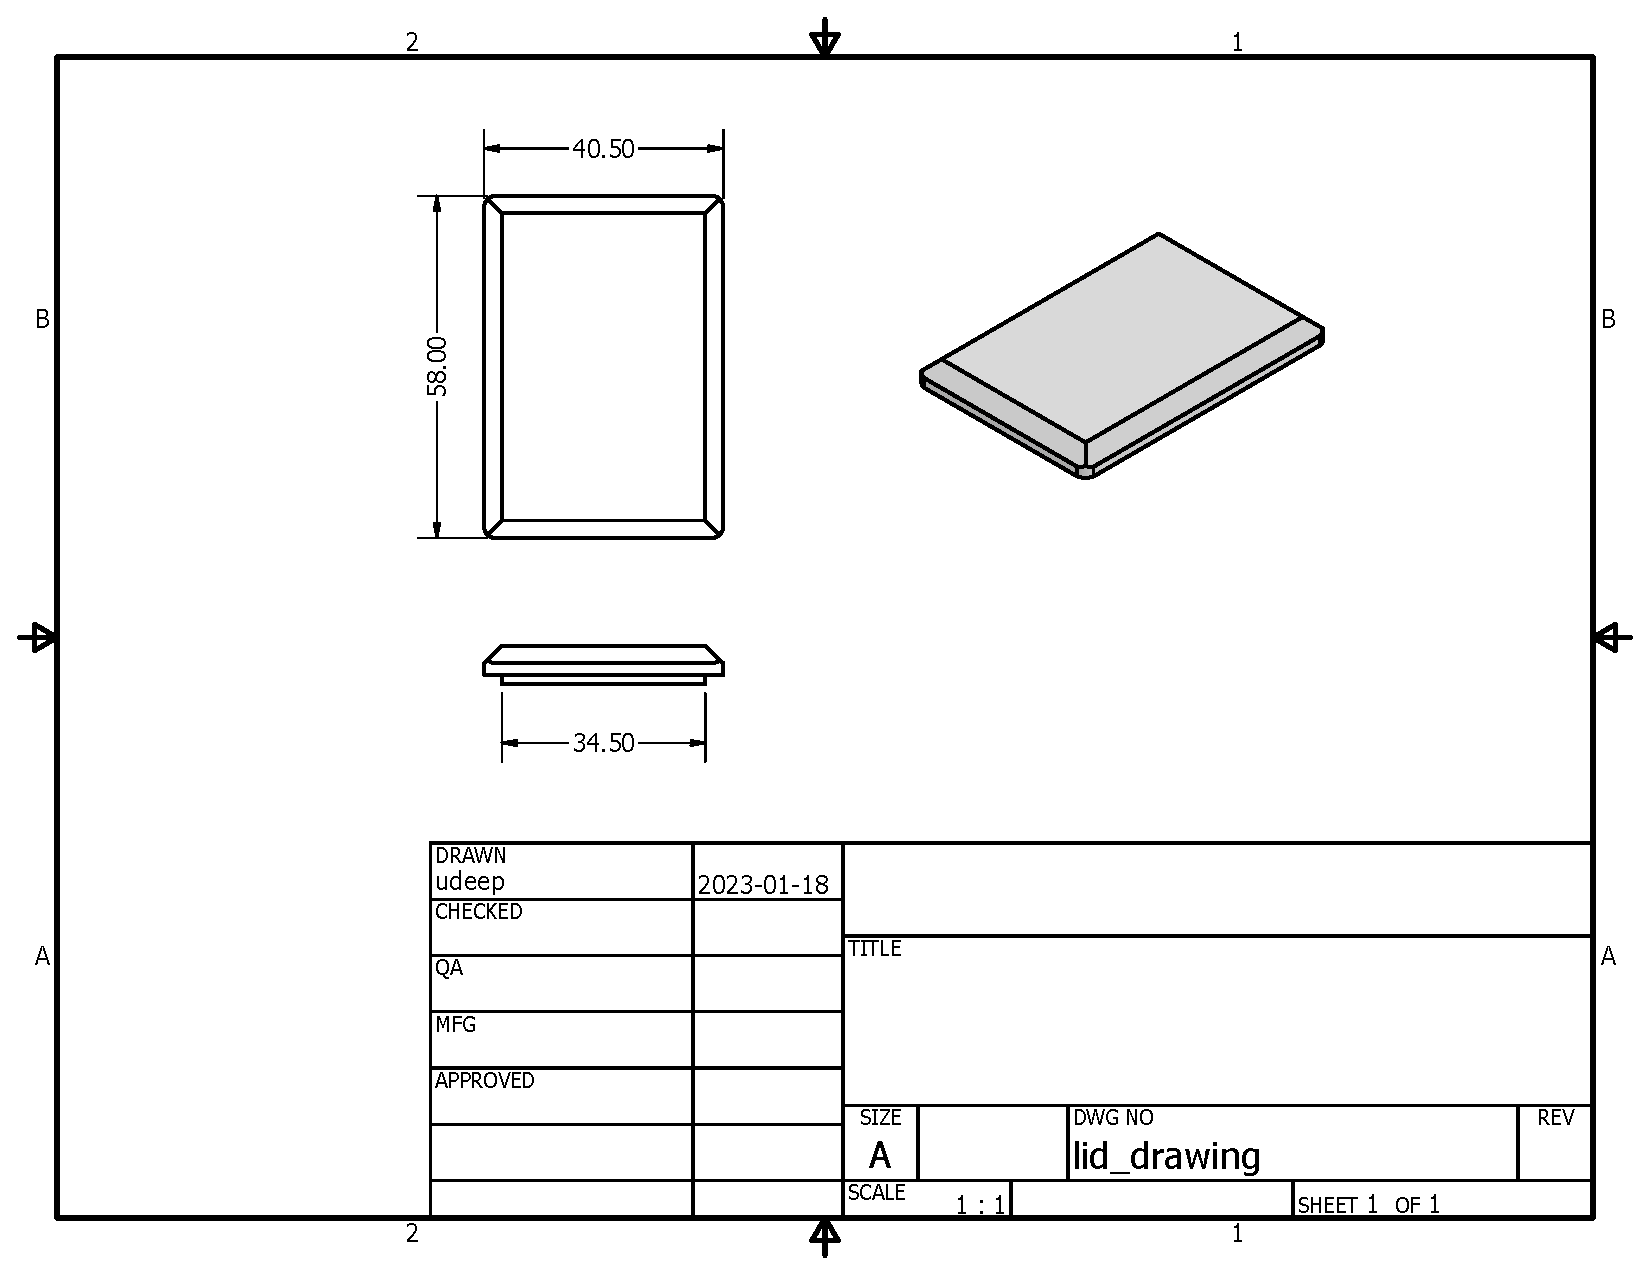
\includegraphics[width=\textwidth,height=\textheight,keepaspectratio]{Lid_drawing.pdf}
\subsection{Assembly}
	\label{appendix:hardware:assembly}

  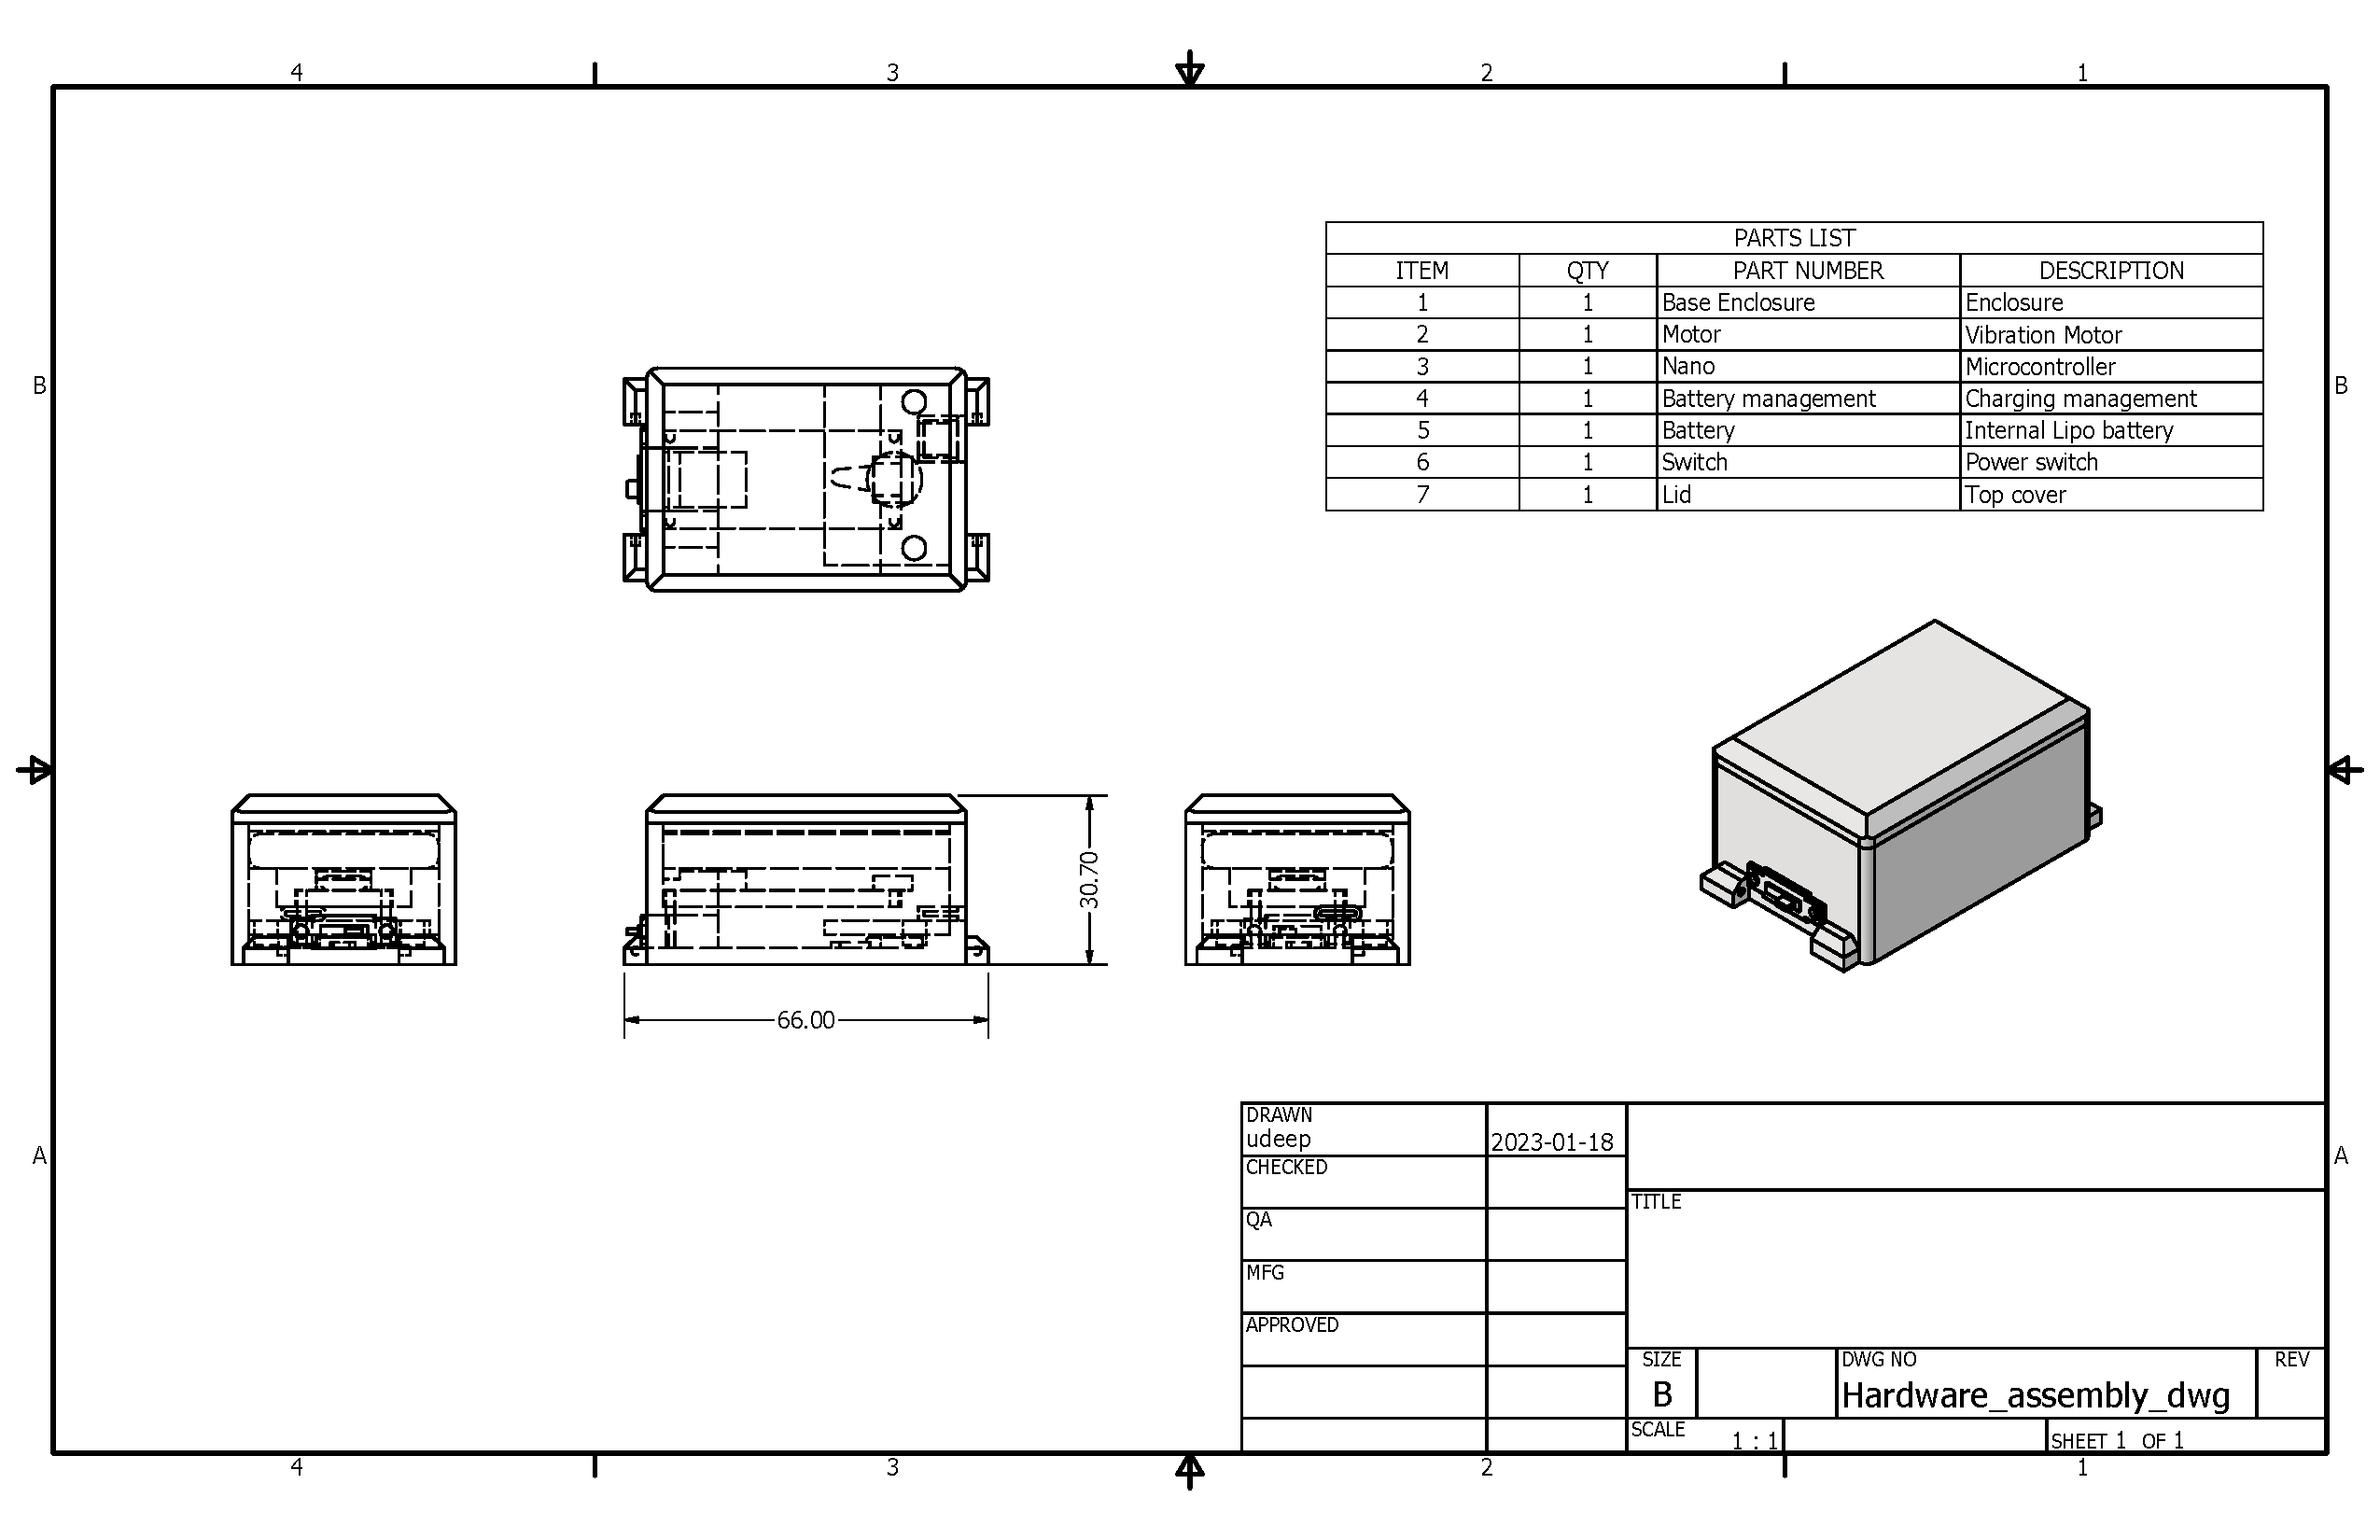
\includegraphics[width=\textwidth,height=\textheight,keepaspectratio]{Assembly_drawing.pdf}

  \section{Reflection}
  \label{appendix:reflection}
  
  
  \begin{enumerate}
    \item \textbf{Limitations of the design} 
    
    Currently the product is quite bulky in terms of size as it is at least 6.5cm in length, 6cm in width, and 3cm in height. It might not seem like much but the final goal was to make the product the size of a small watch instead of a large bulky object. Furthermore, the system cannot function for a long time (at most a day) because the vibration motor and the microphone draw a significant amount of current. Lastly, there are also severe limitations in terms of maintainabilty because once the product is assembled, it cannot be separated. 
    
    If given enough resources, a custom PCB with inbuilt bluetooth, microphone, motor, charging slot, and LiPo support can be acquired. This would make the overall design more efficient, both in terms of power and size. Furthermore, maintainabilty can be increased by changing the enclosure to an insulated metal enclosure with threaded inserts to hold all the components in place.       
    \item \textbf{Other Solutions} 
    
    A potential design solution could have been to use the microphone and processor of a phone to do the sound recording and classification. It would then send a signal to the microcontroller if any distinct sounds were detected. Furthermore, the benefit of this is that the actual hardware could have been smaller and more compact. On another note, this solution has a drawback where the microphone might not be able to hear sounds accurately since the phone might be inside someone's trousers or be too far away from the user (i.e phone is charging). With the above in mind, this solution relies heavily on the smartphone, but having this design work efficiently for all phone types might not be feasible. 

    Another design solution would be to use the microphone on the hardware and to then transmit the sound to the smartphone. From there, the sound will be processed and classified before transmitting the classifed signal back to the microcontroller. With this in mind, this does not have the disadvantage of the smartphone being stuck in trousers as the microphone is near the user while the Synesthesia Wear bracelet is being worn. Lastly, an additional benefit is that the microcontroller can be less powerful and thus more power-efficient. However, the major disadvantage to this is that the smartphone needs to be in range all of the time.    

    In comparison, the current design does all of the processing, recording, and sound classification on the hardware itself which results in a bit more of a bulky bracelet. Furthermore, it only communicates with the smartphone when the user desires to update their preferences. Thus, this is a major advantage of this design because it can work independently (after initial configuration) and does not have to rely on an external smartphone. With this in mind, this was the main reason this design was selected since the product would be independent and self-sufficient.
  \end{enumerate}
  
  \end{appendices}
\end{document}